\documentclass[12pt]{article}
\usepackage{tikz}
\usepackage[subpreambles=true]{standalone}
\usepackage[shortlabels]{enumitem}
\usetikzlibrary{shapes, arrows, decorations.markings}
\usepackage{amsmath,bm,times}
\usepackage{verbatim}
\usepackage{amsfonts}
\usepackage{etex}
\usetikzlibrary{calc,through,intersections}
\usepackage[many]{tcolorbox}
\usepackage{array}
\usepackage{booktabs}
\usetikzlibrary{shadows.blur,shadings}
\pgfdeclarelayer{bg}    % declare background layer
\pgfsetlayers{main,bg}  % set the order of the layers (main is the standard layer)
%-------------------------------------------------MACROS--------------------------------------------------------------------------------
%--------------------------------------------DEMOS-------------------------------------

\newcommand{\mb}{\mathbb}
\newcommand{\tb}[1]{\tilde{\mathbb{#1}}}
\newcommand{\mr}{\mathrm}
\newcommand{\mc}{\mathcal}
\newcommand{\tc}[1]{\tilde{\mathcal{#1}}}
\newcommand{\mbf}{\mathbf}
\newcommand{\msf}{\mathsf}
\newcommand{\Ch}{\mathsf{Ch}}
\newcommand{\mcP}{\mathcal{P}}
\newcommand{\A}{\mathcal{A}}
\newcommand{\Pol}{\mathcal{P}}
\newcommand{\negl}{\mathsf{negl}}
\newcommand{\poly}{\mathsf{poly}}
\newcommand{\la}{\lambda}
\newcommand{\bin}[2]{#1_{n-1}\cdots#1_{#2}}
\newcommand{\Si}{\mathcal{S}}

\newcommand{\set}[1]  {\left\{#1\right\}}
\newcommand{\abs}[1]  {\left|#1\right|}
\newcommand{\odds}[1] {\mathsf{odds}\left(#1\right)}
\newcommand{\floor}[1]{\lfloor #1\rfloor}
\newcommand{\ceil} [1]{\lceil #1\rceil}

\newcommand{\pick} [1] {\overset{#1}{\leftarrow}}
\newcommand{\Adv}{\mathsf{Adv}}
\newcommand{\bind}{\mathsf{bind}}
\newcommand{\hide}{\mathsf{hide}}


\newcommand{\param}{\mathsf{Param}}
\newcommand{\DL}{\mathsf{Dlog}}
\newcommand{\pk}{\mathsf{pk}}
\newcommand{\sk}{\mathsf{sk}}
\newcommand{\Gen}{\mathsf{Gen}}
\newcommand{\Enc}{\mathsf{Enc}}
\newcommand{\Dec}{\mathsf{Dec}}
\newcommand{\accept}{\mathsf{accept}}
\newcommand{\reject}{\mathsf{reject}}
\newcommand{\Sig}{\mathsf{Sig}}
\newcommand{\GenBP}{\mathsf{Gen}_{\mathsf{bp}}}
\newcommand{\Opt}{\mathsf{Opt}}

\newcommand{\VerSig}{\mathsf{Ver}_{\mathsf{sig}}}

%commitment
\newcommand{\Com}  {\mathsf{Com}}
\newcommand{\ck}{\mathsf{ck}}
\newcommand{\Ver}{\mathsf{Ver}}

\newcommand{\view}{\mathsf{view}}



\renewcommand{\vec}[1]{\mathbf{#1}}
\newcommand{\vect}[1]{\overset{\rightarrow}{#1}}

\newcommand{\eatitemspace}{}

\newcommand{\putbox}{\hspace*{\fill}$\Box$}



\newcommand{\Prob}{\mbox{\( \mathbf{ Prob } \)}}

\def\squareforqed{\hbox{\(\blacksquare\)}}
\def\qed{\ifmmode\squareforqed\else{\unskip\nobreak\hfill\penalty50\hskip1em\null\nobreak\hfil\squareforqed\parfillskip=0pt\finalhyphendemerits=0\endgraf}\fi}
\setlength\belowrulesep{0pt}
\setlength\aboverulesep{-1.3pt}
\newcommand{\thickhline}{\midrule[1.2pt]}
\newcommand{\bad}{\mathsf{bad}}


\DeclareMathAlphabet\mathbfcal{OMS}{cmsy}{b}{n}
\newcommand{\VS}{\mathbfcal{VS}}
\newcommand{\VCr}{\mathbfcal{VC}}
\newcommand{\EA}{\mathsf{EA}}
\newcommand{\BB}{\mathsf{BB}}
\newcommand{\BDS}{\mathsf{BDS}}
\newcommand{\VSD}{\mathsf{VSD}}
\newcommand{\ASD}{\mathsf{ASD}}
\newcommand{\VC}{\mathsf{VC}}
\newcommand{\CD}{\mathsf{CD}}
\newcommand{\Admin}{\mathsf{Admin}}
\newcommand{\info}{\mathsf{info}}
\newcommand{\aux}{\mathsf{aux}}
\newcommand{\st}{\mathsf{st}}
\newcommand{\vid}{\mathsf{vid}}
\newcommand{\ch}{\mathsf{Ch}}

\newcommand{\cala}{\mathcal{A}}
\newcommand{\calb}{\mathcal{B}}
\newcommand{\calc}{\mathcal{C}}
\newcommand{\cals}{\mathcal{S}}
\newcommand{\calr}{\mathcal{R}}
\newcommand{\calm}{\mathcal{M}}
\newcommand{\calk}{\mathcal{K}}
\newcommand{\calx}{\mathcal{X}}
\newcommand{\caly}{\mathcal{Y}}
\newcommand{\calf}{\mathcal{F}}
\newcommand{\Z}{\mathcal{Z}}
\newcommand{\calp}{\mathcal{P}}
\newcommand{\calv}{\mathcal{V}}
\newcommand{\call}{\mathcal{L}}
\newcommand{\calo}{\mathcal{O}}
\newcommand{\calu}{\mathcal{U}}
\newcommand{\calt}{\mathcal{T}}

\newcommand{\ZZ}{\mathbb{Z}}
\newcommand{\GF}{\mathbb{GF}}
\newcommand{\GG}{\mathbb{G}}

\newcommand{\Open}{\mathsf{Open}}
\newcommand{\SXDH}{\mathsf{sxdh}}
\newcommand{\Sim}{\mathsf{Sim}}
\newcommand{\td}{\mathsf{td}}
\newcommand{\Prov}{\mathsf{Prov}}
\newcommand{\Vrfy}{\mathsf{Vrfy}}
\newcommand{\crs}{\mathsf{crs}}
%\newcommand{\ch}{\mathsf{ch}}
\newcommand{\opt}{\mathsf{opt}}
\newcommand{\rec}{\mathsf{rec}}
\newcommand{\eid}{\mathsf{eid}}
%\newcommand{\hash}{\mathsf{hash}}



\newcommand{\NIZK}{\mathsf{NIZK}}

\newcommand{\name}{PoWorK}
\newcommand{\steps}{\msf{Steps}}


\newcommand{\Setup}{\mathbf{Setup}}
\newcommand{\Cast}{\mathbf{Cast}}
\newcommand{\Tally}{\mathbf{Tally}}
\newcommand{\Result}{\mathbf{Result}}
\newcommand{\Verify}{\mathbf{Verify}}

\newcommand{\blt}{\mathbf{blt}}
\newcommand{\ta}{\mathbf{ta}}

%%%%%%%%%%%%%%%%%%%%%%%%%%%%%%%%%%%%%%%%%%%%
%-------------------------ENVIRONMENTS---------------------------------------------------

\newenvironment{proofsketch}{\noindent\textit{Proof sketch:}}{\putbox}
\newenvironment{PhDproof}{\noindent {\em Proof:}}{\putbox}
%
\newenvironment{boxfig}[2]{%
     \begin{figure}[h!]
     \newcommand{\FigCaption}{#1}
     \newcommand{\FigLabel}{#2}
%     \vspace{-0.25cm}
     \begin{center}
       \begin{small}
         \begin{tabular}{@{}|@{~~}l@{~~}|@{}}
           \hline
           \rule[-1.5ex]{0pt}{1ex}\begin{minipage}[b]{.9\linewidth}
             \vspace{1ex}
             \smallskip
             }{%
           \end{minipage}\\
           \hline
         \end{tabular}
       \end{small}
%       \vspace{-0.25cm}
      \caption{\FigCaption}
%       \figlab{\FigLabel}
     \end{center}
     \vspace{-0.5cm}
   \end{figure}
}
%
%
\newtcolorbox{phdshadebox}[1][]{
  enhanced, %drop shadow east,
  boxrule=1.5pt,arc=.3em,boxsep=-1mm,
  left=.5em,right=.5em,top=5pt,bottom=5pt,
  colback=white,#1
}
%
\newenvironment{shadowfig}[2]{%
     \begin{figure}[H]
     \newcommand{\FigCaption}{#1}
     \newcommand{\FigLabel}{#2}
     \begin{phdshadebox}
%
\begin{center}
\begin{small}
\begin{minipage}{0.95\linewidth}
\medskip
%
}{
%
\smallskip
\end{minipage}
\end{small}
\end{center}
\end{phdshadebox}
\smallskip
  \caption{\FigCaption}
    \label{\FigLabel}
\end{figure}
}


\newenvironment{experiment}{
%\medskip
\begin{center}\begin{boxedminipage}{\linewidth}}{\end{boxedminipage}\end{center}
%\medskip
}

%
\newtcolorbox{shadebox}[1][]{
  enhanced,drop shadow shouthwest,
  boxrule=1pt,arc=1pt,boxsep=0pt,
  left=.5em,right=.5em,top=1ex,bottom=1ex,
  colback=white,#1
}
%
%
\newtcolorbox{eqbox}[1][]{
  enhanced, %drop shadow east,
  boxrule=1pt,arc=2mm, outer arc=2mm,boxsep=-1mm,colframe=mygray!20!black,
  left=.5em,right=.5em,top=10pt,bottom=10pt,halign=center,fuzzy shadow={2pt}{-2pt}{0pt}{0.2pt}{mygray},%drop large lifted shadow,
  colback=white, attach boxed title to top center={yshift=-0.8mm},#1
}
%
\newtcolorbox{stepbox}[1][]{
  enhanced,%drop shadow shouthwest,
  boxrule=0.75pt,arc=1pt,boxsep=0mm,
  left=.25em,right=.25em,top=10pt,bottom=10pt, attach boxed title to top center={yshift=-0.8mm},
  colback=white,#1
}

\tikzset{% 
    trustee/.style={%
        draw,align = center, text width = 32pt, text height = 20pt,line width=1.2pt,rounded corners=2pt,fill = white, 
        blur shadow={shadow xshift=2pt}
        }
}

\tikzset{% 
    voter/.style={%
        draw,circle,align = center, text width = 18pt, line width=1.2pt,fill = white, blur shadow={shadow xshift=1pt}
    }
}
\tikzset{% 
    human/.style={%
        draw,circle,align = center, text width = 16pt, line width=1.2pt,fill = white, drop shadow={shadow xshift=2.5pt, shadow yshift=-1.5pt, fill=mygray}
    }
}

\tikzset{% 
    SD/.style={%
        draw,align = center, text width = 27pt, text height = 15pt,line width=1.2pt,rounded corners=2pt,fill = white, 
       drop shadow={shadow xshift=2.5pt, shadow yshift=-1.5pt, fill=mygray}
        }
}
\tikzset{
sarrow/.style={
  draw,
  double arrow,
  text width=15pt,
  text height=10pt,
  fill=black
  }}
%%extractor
\newcommand{\Ext}{\mathsf{Ext}}
\newcommand{\pok}{\mathit{PoK}}
\newcommand{\pow}{\mathit{PoW}}

%%puzzle
\newcommand{\true}{\mathsf{true}}
\newcommand{\false}{\mathsf{false}}
\newcommand{\puz}{\mathsf{puz}}
\newcommand{\soln}{\mathsf{soln}}
\newcommand{\PuzSys}{\mathsf{PuzSys}}
\newcommand{\GenP}{\mathsf{GenPuz}}
\newcommand{\SolveP}{\mathsf{Solve}}
\newcommand{\Sample}{\mathsf{Sample}}
\newcommand{\SampleP}{\mathsf{SampleSol}}
\newcommand{\VerP}{\mathsf{Verify}}
\newcommand{\PuzzleS}{\mathcal{PS}}
\newcommand{\HardS}{\mathcal{HS}}
\newcommand{\SolutionS}{\mathcal{SS}}
\newcommand{\Params}{\mathsf{params}}
\newcommand{\LSB}{\mathsf{LSB}}
\newcommand{\CS}{\mathcal{CS}}

\newcommand{\AAA}{\mathcal{A}}
\newcommand{\BBB}{\mathcal{B}}
\newcommand{\EEE}{\mathsf{E}}
\newcommand{\FFF}{\mathcal{F}}
\newcommand{\CCC}{\mathcal{C}}
\newcommand{\DDD}{\mathcal{D}}
\newcommand{\III}{\mathcal{I}}
\newcommand{\RRR}{\mathcal{R}}
\newcommand{\LLL}{\mathcal{L}}
\newcommand{\KKK}{\mathcal{K}}
\newcommand{\PPP}{\mathsf{P}}
\newcommand{\VVV}{\mathsf{V}}
\newcommand{\SSS}{\mathcal{S}}
\newcommand{\XXX}{\mathcal{X}}
\newcommand{\ZZZ}{\mathcal{Z}}

\newcommand{\Pone}{\mathsf{P1}}
\newcommand{\Ptwo}{\mathsf{P2}}
\newcommand{\KK}{\mathsf{K}}
%\newcommand{\B}{\mathcal{B}}

\newcommand{\ignore}[1]{\relax} 
%------------------NOTES-----------------------------
\newif\ifNotes
%\Notestrue
\Notesfalse
\newcommand{\note}[1]{\ifNotes\textcolor{blue}{\textsc{Note}: #1}\else{}\fi}
%

\renewcommand{\figurename}{\textsc{Figure}}
\renewcommand{\tablename}{\textsc{Table}}
\newcolumntype{M}[1]{>{\centering\arraybackslash}m{#1}}
\definecolor{mygray}{RGB}{200,200,200}
\definecolor{lightgray}{RGB}{220,220,220}
\definecolor{darkgray}{RGB}{100,100,100}
\definecolor{ultradarkgray}{RGB}{30,30,30}
\definecolor{ultralightgray}{RGB}{230,230,230}

\author{Tamara Finogina}
\title{Exploring boundaries of privacy in e2e verifiable e-voting systems.}
\date{}
\DeclareMathOperator{\exec}{EXEC}
\DeclareMathOperator{\vsd}{VSD}
\DeclareMathOperator{\asd}{ASD}
\DeclareMathOperator{\ea}{EA}
\DeclareMathOperator{\bb}{BB}
\DeclareMathOperator{\voc}{VC}

% for double arrows a la chef
% adapt line thickness and line width, if needed
\tikzstyle{vecArrow} = [thick, decoration={markings,mark=at position
   1 with {\arrow[semithick]{open triangle 60}}},
   double distance=1.4pt, shorten >= 5.5pt,
   preaction = {decorate},
   postaction = {draw,line width=1.4pt, white,shorten >= 4.5pt}]
\tikzstyle{innerWhite} = [semithick, white,line width=1.4pt, shorten >= 4.5pt]
\renewcommand\labelenumi{(\theenumi)}
\newcommand{\mx}[1]{\mathbf{\bm{#1}}} % Matrix command
\newcommand{\vc}[1]{\mathbf{\bm{#1}}} % Vector command

% We need layers to draw the block diagram
\pgfdeclarelayer{background}
\pgfdeclarelayer{foreground}
\pgfsetlayers{background,main,foreground}

% Define a few styles and constants
\tikzstyle{sensor}=[draw, text width=2em, 
    text centered, minimum height=2.5em]
 \tikzstyle{s}=[draw, text width=6em, 
    text centered, minimum height=5em]
 \tikzstyle{sim}=[draw, text width=8em, 
    text centered, minimum height=6em]
\tikzstyle{ann} = [above, text width=5em]
\tikzstyle{a} = [sensor, text width=6em,
    minimum height=8em, rounded corners]
 \tikzstyle{v} =[circle, thick, minimum size=0.8cm, draw=black]
  \tikzstyle{vv} =[circle, thick,  dashed,draw=black!50]
\def\blockdist{2.3}
\def\edgedist{2.5}
\begin{document}
\maketitle
\section{Preliminaries} 
\subsection{Notations}
Through this paper, we denote $\lambda$ as the security parameter. We use $negl(\lambda)$ to denote a negligible function in $\lambda$, i.e., it always holds that $negl(\lambda) < \frac{1}{\lambda^c}$ for any $0<c \in \mathbb{Z}$ for sufficient large $\lambda$. 
\section{E-voting model}
\subsection{Syntax} 
An e-voting system is an interactive protocol $\Pi$ among a set of entities and voters, that takes  voters' preferences as and input and aims to return a tally. \\

In this modelling, the election system involves five types of entities, the voters $V_1, \dots , V_n$, possibly equipped with the voting supporting device ($\vsd$) and the auditing supporting device ($\asd$), the election authority ($\ea$), the vote collector ($\voc$), the trustee ($T$), and the bulletin board ($\bb$) whose only role is to provide storage for the election transcript for the purpose of verification. 
\begin{enumerate}
\item $\bb$ is completely passive and is only writeable by the $\voc$ and readable by anyone. 
\item Voters submit their votes by engaging in the ballot casting protocol to the $\voc$ and they are not allowed to interact with each other. 
\item $\voc$ only role is to collect votes and write them to $\bb$
\item $T$ is responsible for computing the tally and announcing the election result.
\item $\ea$ - prepares all the election setup information and distributes the voters' ballots.
\end{enumerate}
\begin{figure}
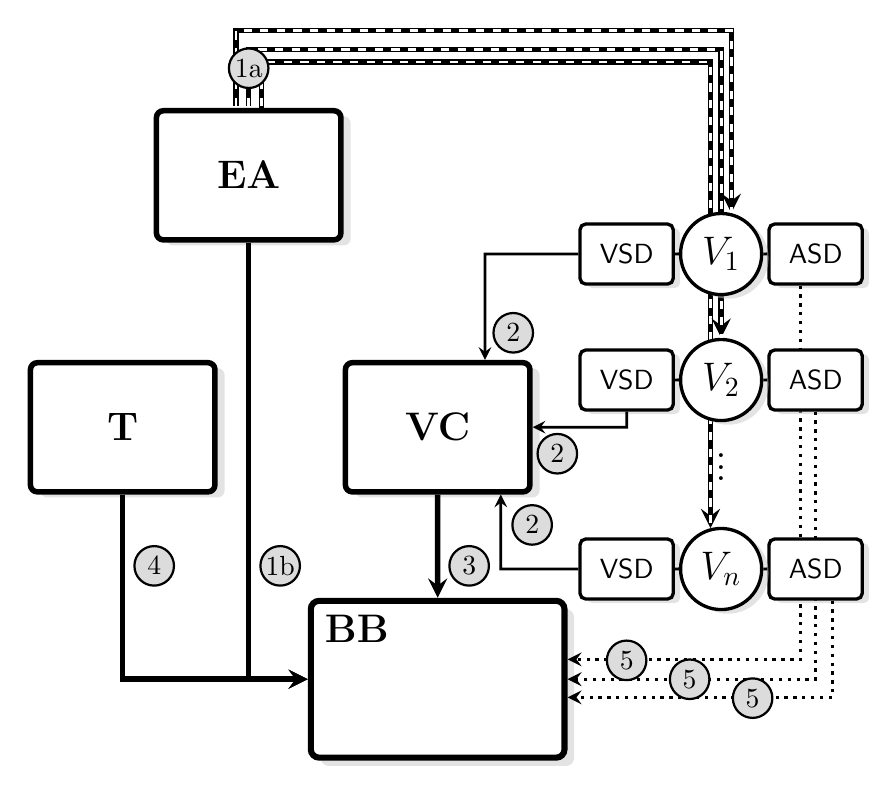
\begin{tikzpicture}[scale=0.8]
  %\draw[step=10pt,gray,very thin] (0,0) grid (30,30);
  
  %\draw[step=1pt,thick] (25,15) rectangle (28,16.5) ;
  \node[draw, align = center, text width = 60pt, text height=40pt,rounded corners=2.5pt,line width=2pt,fill = white, drop shadow={shadow xshift=3.5pt, shadow yshift=-2pt, fill=mygray}]  (EA) at (7,24) {};
  
    \node[draw, align = center, text width = 60pt, text height=40pt,rounded corners=2.5pt,line width=2pt,fill = white, drop shadow={shadow xshift=3.5pt, shadow yshift=-2pt, fill=mygray}]  (VC) at (10,20) {};
    
      \node[draw, align = center, text width = 60pt, text height=40pt,rounded corners=2.5pt,line width=2pt,fill = white, drop shadow={shadow xshift=3.5pt, shadow yshift=-2pt, fill=mygray}]  (T) at (5,20) {};
    
  \node at (EA) {\Large{\textbf{EA}}};
 \node at (VC) {\Large{\textbf{VC}}};
  \node at (T) {\Large{\textbf{T}}};
%



 %
% \node (CD) at (11,23.5) {};

 
\node[draw, fill =white, align = center, text width = 85pt,text height=50pt,rounded corners=3pt,line width=2.2pt, drop shadow={shadow xshift=3.5pt, shadow yshift=-3pt, fill=mygray}] (BB) at (10,16) {}; 

 \node[below right, inner sep=6pt] at (BB.north west) {\Large{\textbf{BB}}};
 
  \draw[->,>=stealth,line width=2pt] (VC)--(BB) ;
    \draw[->,>=stealth,line width=2pt] (EA.south) |- (BB.west);
    \draw[->,>=stealth,line width=2pt] (T.south) |- (BB.west);

 
 %
  \node[SD](VSD1) at (13,22.75) {};
        \node[SD](VSD2) at (13,20.75) {};
     \node[SD](VSDn) at (13,17.75) {};
   
      \node[SD](V-ASD1) at (16,22.75) {};
   \draw[->,>=stealth,dotted,very thick] ([xshift=-80pt]V-ASD1)|-([yshift=25pt]BB);
      \node[SD](V-ASD2) at (16,20.75) {};     
      \draw[->,>=stealth,dotted, very thick] (V-ASD2)|-(BB);      
           \node[SD](V-ASDn) at (16,17.75) {};
         \draw[->,>=stealth,dotted, ,very thick] ([xshift=40pt]V-ASDn)|-([yshift=-25pt]BB);
         
         
     \node[align = center, text width = 22pt, thick]  (Vdots) at (14.5,19.5) {\Large{$\vdots$}}  ; 
     %
         %
    \node[human]  (Vn) at (14.5,17.75) {\Large{$V_n$}}  ;      
   \node at (VSDn) {{\textsf{VSD}}};
   \node at (V-ASDn) {{\textsf{ASD}}};
   \draw[->,>=stealth,line width=2pt] (7.2,25)--(7.2,25.8) -|([xshift=-60pt]Vn) ;
 \draw[-,>=stealth,dashed,line width=1pt,color=white] (7.2,25.1)--(7.2,25.8) -|([xshift=-60pt,yshift=-25pt]Vn) ;

         %         
    \node[human]  (V2) at (14.5,20.75) {\Large{$V_2$}}  ; 
   \node at (VSD2) {{\textsf{VSD}}};
   \node at (V-ASD2) {{\textsf{ASD}}};
  \draw[->,>=stealth,line width=2pt] (7,25.1)--(7,26) -|(V2) ;
    \draw[-,>=stealth,dashed,line width=1pt,color=white] (7,25.1)--(7,26) -|([yshift=-25pt]V2) ;
%         
   \node[human]  (V1) at (14.5,22.75) {{\Large{$V_1$}}}  ; 
   \node at (VSD1) {{\textsf{VSD}}};  
   \node at (V-ASD1) {{\textsf{ASD}}};
   \draw[->,>=stealth,line width=2pt] (6.8,25.1)--(6.8,26.3) -|([xshift=25pt]V1) ;
  \draw[-,>=stealth,dashed,line width=1pt,color=white] (6.8,25.1)--(6.8,26.3) -|([xshift=25pt,yshift=-25pt]V1) ;

 %

   %
\draw [->,>=stealth,line width=1pt] (V-ASD1)--(V1) -- (VSD1)-|([xshift=55pt]VC) ;
\draw [->,>=stealth,line width=1pt] (V-ASD2)--(V2) -- (VSD2)|-(VC) ;
\draw [->,>=stealth,line width=1pt] (V-ASDn)--(Vn)-- (VSDn)-|([xshift=60pt]VC) ;

 \node[draw,circle,text width=6pt,line width=0.8pt,fill = lightgray] (C1b) at (7.5,17.8) {};
 \node at (C1b) {1b} ;
 %
  \node[draw,circle,text width=6pt,line width=0.8pt,fill = lightgray] (C1a) at (7,25.7) {};
 \node at (C1a) {1a} ;
 %
  \node[draw,circle,text width=6pt,line width=0.8pt,fill = lightgray] (C3) at (5.5,17.8) {};
 \node at (C3) {4} ;
  %
  \node[draw,circle,text width=6pt,line width=0.8pt,fill = lightgray] (C2b) at (10.5,17.8) {};
 \node at (C2b) {3} ;
 %
  \node[draw,circle,text width=6pt,line width=0.8pt,fill = lightgray] (C41) at (13,16.3) {};
 \node at (C41) {5} ;
 %
  \node[draw,circle,text width=6pt,line width=0.8pt,fill = lightgray] (C42) at (14,16) {};
 \node at (C42) {5} ;
 %
  \node[draw,circle,text width=6pt,line width=0.8pt,fill = lightgray] (C4n) at (15,15.7) {};
 \node at (C4n) {5} ;
 
   \node[draw,circle,text width=6pt,line width=0.8pt,fill = lightgray] (C21) at (11.2,21.5) {};
 \node at (C21) {2} ;
 %
  \node[draw,circle,text width=6pt,line width=0.8pt,fill = lightgray] (C22) at (11.9,19.58) {};
 \node at (C22) {2} ;
 %
  \node[draw,circle,text width=6pt,line width=0.8pt,fill = lightgray] (C2n) at (11.5,18.45) {};
 \node at (C2n) {2} ;
\end{tikzpicture}
    \caption{The interaction among the entities in an e-voting execution. The dotted lines denote read-only access to the BB. The dashed arrows denote channels for voters' private inputs distribution. Annotation: (1a): distribution of voter's private inputs; (1b): pre-election BB data; (2): vote casting; (3): writing votes to BB; (4)  post-election BB data; (5): auditing.}
        \label{interaction}
\end{figure}
Protocols
An e-voting system $\Pi$ is a quintuple of algorithms and protocols  \textbf{(Setup, Cast, Tally, Result, Verify)} specified as follows:
\begin{enumerate}
\item The algorithm \textbf{Setup} is executed by the $\ea$ and $T$ separately. During the setup phase $\ea$ generates $\Pi$'s public parameters $Pub$ (which include $P, V, U$) and the voters' secrets $s_1, \dots , s_n$. The part of the algorithm during which $\ea$ distributes secrets among voters is defined as \textbf{Registration}. At the same time, $T$ generates pre-election $\bb$ data and posts it on $\bb$.
\item The interactive protocol \textbf{Cast} is executed between three parties, the voter $V_l$, the $\bb$ and the $\voc$. During this interaction, the voter uses $\vsd$, his secret $s_l$ and an option $U_l$ to generate the ballot $b_l$ and sends this ballot to $\voc$. Upon successful termination, $\voc$ posts ballot $b_l$ to $\bb$ and the voter $V_l$ receives a receipt $\alpha_l$.
\item The algorithm \textbf{Result} is executed by $T$ and outputs the result $\tau$ for the election or returns $\perp$ in case such result is undefined.
\item  The algorithm \textbf{Verify} outputs a value in $\{0,1\}$, where  $\alpha$ is a voter receipt (that corresponds to the voter's output from the \textbf{Cast} protocol).
\end{enumerate}
In some e-voting systems \textbf{Registration} part is omitted and voters are expected to receive their credentials via secure channel such as post mail, pulling place etc.
\subsection{Correctness of a system}
We say that a system $\Pi$ has (perfect) correctness, if for any honest execution of any subset of not abstained voters that results in a public transcript $\tau$, where the voters $V_1, . . . , V_n$ cast votes for options $U_1, . . . , U_n$, it holds that $Result(\tau) = f(U_1,...,U_n)$, where $f(U_1,...,U_n)$ is the m-vector whose i-th location is equal to the number of times a candidate $P_i \in \{P_1,\dots, P_m\}$ was chosen in the candidate selections $U_1, . . . , U_n$.
\section{Privacy with respect to entities}
\subsection{EA only}
If $\ea$ is trusted and all other entities ($T,\vsd,\voc$) are corrupted ($\bb$ is completely passive and simply posts all information received from $\voc$) it is impossible to preserve voter's privacy. \\\\
Proof:\\\\
Suppose there is some e-voting system $\Pi$ which doesn't allow any adversary to learn anything about individual voters' intents in case when only $\ea$ is trusted. $\mathcal{A}$ strategy is to calculate tally after every vote submission and compare it with the previous tally to learn the voter's intent. Due to a correctness, $\Pi$ should be able to produce meaningful election tally for any turnout, including just one voter. Since an adversary $\mathcal{A}$ controls a trustee $T$, he should be able to compute results after very first cast procedure is done. This means that either $\mathcal{A}$  may learn voters' choices one by one or $\Pi$ fails to produce results for any subset of abstained voters  and therefore is not correct. 
\subsubsection{EA + VC}
 It's not enough for privacy, an adversary can perform exactly the same attack as for '$\ea$ only case'
\subsubsection{EA + T}
Private. Example: Demos 
\subsubsection{EA + VSD}
 In such case $\Pi$ can be private, since it's enough to have a trusted $\vsd$ for preserving voters' privacy.
\subsection{VSD only:}
 VSD is trusted, all other entities ($T,\ea,\voc$) are controlled by an adversary. $\bb$ is completely passive and simply posts all information received from $\voc$. 
Consider the following e-voting system $\Pi$:
\begin{enumerate}
 \item $\ea$ generates a large random number $R$ and commitments bases $g,h$. Also $\ea$ picks a random id  $x_i$ for every candidate $cand_i$. $R,g,h, \{cand_i,x_i\}$  - $\Pi$'s public information. 
 \item each voter submits vis $\vsd$ a perfectly hiding commitment $g^{x_i}h^{r_l}$, where $r_l$ is a random number less than R picked by $\vsd$. 
 \item after the last voter cast his vote, $\vsd$ submits a commitment $g^{x_{abs}}h^{r_{vsd}}$, where $x_{abs}$ corresponds to the abstain option and $r_{vsd} = R - \sum_{l=0}^{l=n}r_l$, n - number of voters.  
 \item $T$ computes the product of all hiding commitments and opens the result.
 \end{enumerate}
  In order to break voters' privacy, an adversary has to break perfectly hiding commitments. 
\subsection{VC only}
  Impossible.   An adversary can perform exactly the same attack as for '$\ea$ only case.
\subsubsection{VC + T}
 Due to the assumption that voters are not able to collaborate for protecting their privacy and all complex math operation performed by $\vsd$ or $\ea$, it's impossible to have privacy in this case. A voter provides $\vsd$ with an input which is either in a plain text or calculated by $\ea$ line and therefore immediately gives away his choice.
\subsubsection{VC + VSD}
    In such case $\Pi$ can be private, since it's enough to have a trusted $\vsd$ for preserving voters' privacy. 
\subsubsection{VC + EA}
 Impossible. See the EA + VC  case for details. 
\subsection{T only}
  Impossible. Same reasoning as VC + T case.
\subsubsection{T + VC}
   seems meaningless
\subsubsection{T + VSD}
    In such case $\Pi$ can be private, since it's enough to have a trusted $\vsd$ for preserving voters' privacy. 
\subsubsection{T + EA}
   Private. See the EA + T case for details. 
\section{Strict privacy notion}
Voter privacy implies that a voter is capable of casting his own vote secretly and freely without letting others' parties, namely an adversary, to learn some information about his preferences or interfere in it.\\

In general, the goal of the adversary who attacks voter privacy is to learn some information about the candidate selections of the honest voters. We define an attack against voters privacy successful, if there is an election result*, for which an adversary is capable of distinguishing how the honest voters voted while it can observe the whole e-voting network** and corrupt some part of honest voter and some entities and also has access to honest voters' receipts. \\

*Obviously, it doesn't include trivial election results, where all voters voted for the same option. \\
**Except channels that are marked as untrappable. \\



In this section we use term strict privacy to imply that an adversary interacts with an e-voting system on behalf of all voters and there is no such thing as honest voters. In general, strict privacy means that even the person who cast a vote can not break his own privacy after the Cast phase is completed. \\

We formally define the strict voter privacy via a Voter Privacy game, denotes as $G_{strict,<honest~entities>}^{\mathcal{A}, Sim}(1^{\lambda})$, that is played between an adversary $\mathcal{A}$ and a challenger $\mathcal{C}$, that takes as input the security parameter $\lambda${\color{red}*} and returns 1 or 0 depending on whether the adversary wins.  Also, $\mathcal{A}$ is  allowed to corrupt some entities. The choice of the corrupted parties splits the Voter Privacy game into two different scenarios. All meaningful* cases of collusion fall into two scenarios: (1) entities ($\ea$, $T$) are hones and (2) $\vsd$ is honest. \\
{\color{red} Thomas, do you think that m and n (the number of candidates and the number of voters)  should be added as the input parameters to the Voter Privacy game? Now, it's up to adversary to define an election parameters. }\\
*In cases where only $\ea$ or $T$ can be trusted it is not possible to have voter privacy. \\

 According to the game rules, an adversary is allowed to define an election parameters, act on behalf of all voters and corrupted entities. During the game $\mathcal{C}$ plays the role of honest parties and returns to the adversary simulated and real view in order defined by a coin $a$ (If $a=0$, $\mathcal{C}$ returns $(simulated\_view,real\_view)$ and  $(real\_view,simulated\_view)$ otherwise). A challenger flips the coin $a$ only once, before interaction with $\mathcal{A}$.  Note that the result of the game heavily depends on an efficiency of the simulator that is used by the challenger for producing a simulated view. \\

We will show that the notion of strict privacy is the weakest level of privacy that contradicts end-to-end verifiability. 

\subsection{$\ea$ and $T$ are honest: $G_{strict,\ea,T}^{\mathcal{A}, Sim}(1^{\lambda})$}
In the case of trusted $\ea$ and $T$,  $\mathcal{C}$ uses a simulator $Sim$ to generate a fake credentials so an adversary would not be able to distinguish the result of the \textbf{Cast} protocol with his intent and real credentials and with another candidates selection and fake credential given as input. \\

$\mathcal{C}$  behaviour in the  $G_{strict,\ea,T}^{\mathcal{A}, Sim}(1^{\lambda})$ game captures the ability of a honest voter to lie about his vote in code-based e-voting schemes. Suppose, an adversary  makes a voter V to cast his vote for an option $U_{\mathcal{A}}$ instead of the voter's original intent $U_{V}$.  V still can cast vote for the option $U_{V}$ and fake his credentials in a way that his actual receipt would correspond to the option $U_{\mathcal{A}}$. If by faking credential V can fool an adversary into believing that he cast vote for $U_{\mathcal{A}}$, his privacy is preserved. \\

For every vote that an adversary cast, $\mathcal{C}$ creates a fake voter who cast exactly the same vote. Every round the sum of an adversarial vote and an challenger's vote would give $U_{\mathcal{A}}$ + $U_{V}$. An actual vote distribution depends on the credentials choice. If $\mathcal{A}$ uses real credentials he votes for the $U_{\mathcal{A}}$ and  $\mathcal{C}$ --  for the $U_{V}$. Otherwise , $\mathcal{A}$' vote corresponds to  the  option $U_{V}$  and  $\mathcal{C}'$ vote to the $U_{\mathcal{A}}$. $\mathcal{A}$ is provided with both credentials real and fake in order defined by $\mathcal{C}$ 's coin $a$. If $a=0$ $\mathcal{C}$  returns $(fake\_credentials,real\_credentials)$ and $(real\_credentials,fake\_credentials)$ otherwise. An adversary tries to guess the coin $a$. $\mathcal{A}$ may stop the game in any moment  {\color{red}*}. \\
{\color{red} Not really. An adversary can not stop the game in the moment after he cast his vote and before $\mathcal{C}$ posts a fake voter's vote.}

   \begin{figure}[h!]
 \includestandalone[mode=buildnew]{figures/figure1}
        \caption{$G_{strict,\ea,T}^{\mathcal{A}, Sim}(1^{\lambda})$}
        \label{EAT is honest}
\end{figure}
In the game   $G_{strict,\ea,T}^{\mathcal{A}, Sim}(1^{\lambda})$ , an adversary $\mathcal{A}$ interacts with the challenger $\mathcal{C}$ on behalf of all voters, $\voc$ and $\vsd$. $\mathcal{C}$ plays the role of $\ea$ and $T$. $\bb$ is completely passive and represents a publicly viewed database. \\\\
After an adversary  $\mathcal{A}$  defined an election parameters, $\mathcal{C}$  doubles the voters, computes setup data and starts the election. This duplication of voters is needed because $\mathcal{C}$ would post another ballot for every adversarial's cast ballot. If $\mathcal{A}$ abstains, $\mathcal{C}$ abstains as well. During the game, we will refer to duplicated voters as fake ones. \\\\
$\mathcal{A}$ 1) picks and sends two options $U_{i_1},U_{i_2}$ {\color{red}*} to the challenger $\mathcal{C}$. One of the options $U_{i_1}, U_{i_2}$ is his intent, the other -- the option that the challenger would use in order to produce an indistinguishable from the intent's ballot and receipt view*. After sending options, 2) $\mathcal{A}$ runs the   \textbf{Registration} as if he is $V_i$. $\mathcal{C}$ creates a fake credentials $\tilde{s_i}$ and 3) generates real credentials $s_i$ for him. 4) $\mathcal{C}$ responds $\mathcal{A}$ with a pair of credentials $s_0,s_1$, where one of the credentials are real and the other were generated using the simulator $Sim$ in a such way, that no matter what credential $s_0$ or $s_1$ $\mathcal{A}$ uses to cast a vote for $U_{i_1}$, the produced ballot would also correspond to the result of the \textbf{Cast} protocol for an option $U_{i_2}$ with the other credentials and vice versa. If 5) $\mathcal{A}$ choses to post the ballot $b_i$ to $\bb$, 6) $\mathcal{C}$  posts exactly the same ballot to $\bb$ on behalf of the fake voter. When $\mathcal{A}$ stops the election, 7) $\mathcal{C}$ posts the tally $\tau$ **. \\\\
{\color{red} *Haven't thought about the case when  $U_{i_1} = U_{i_2}$. Should the challenger return same credentials or Sim would generate something different? On the one hand, it's fine for a Sim to generate exactly the same credentials. If it generates something different, the result of the game depends on how good Sim is. On the other hand, case $U_{i_1} = U_{i_2}$ is a bit weird. This game tries to capture a way how a honest voter fakes his credentials to convince $\mathcal{A}$ that he voted as he was told. There is no point in faking anything if you may as well give back real stuff. } \\
Remarks:\\
*If  $\mathcal{C}$ succeeds, $\mathcal{A}$ wouldn't be able to say whether his ballot and receipt corresponds to $U_{i_1}$ or $U_{i_2}$ and $\bb$ would contain both ballots (one for the option $U_{i_1}$ ,the other for the option $ U_{i_2}$) so the tally wouldn't reveal any information. Example: if $\mathcal{A}$  picks real credential for the voter $V_i$ then he casts a vote for the option  $U_{i_1}$ , at the same time exactly the same ballot posted $\mathcal{C}$ on behalf of the fake voter $\tilde{V_i}$ would correspond to the fake credentials and the option $U_{i_2}$. In this case $\mathcal{A}$  voted for $U_{i_1}$. Else if $\mathcal{A}$ picks fake credentials and tries to vote for the option $U_{i_1}$,  his ballot corresponds to the real credentials and  the option $U_{i_1}$. At the same time, exactly the same ballot posted $\mathcal{C}$ on behalf of the fake voter $\tilde{V_i}$ would correspond to the fake credentials  and the option $U_{i_1}$. So $\mathcal{A}$  voted for $U_{i_1}$. If this definition holds,  $\mathcal{A}$ has no idea whom he voted for. \\
** The tally $\tau$ is posted only if all ballots are correctly formed: were produced with one of the provided credentials, for the candidate $U_{i_1}$, for every cast ballot there is a duplicate, etc. \\
\textcolor{red}{Thomas, may be you are right and here I should use two sets of votes that sums to the same tally. I'm not entirely sure, though. This approach seems quite similar to the 'only $\vsd$ is trusted' case.  Here $\mathcal{A}$ can't say wether he voted for $U_{i_1}$ and $\mathcal{C}$ for $U_{i_2}$ or vice versa. On the one hand, he knows options $U_{i_1}$  and $U_{i_2}$ and just couldn't link them with voters.  $U_{i_1}$ and $U_{i_2}$ are defined by $\mathcal{A}$ and keep changing during the game. Generally, in order to save my privacy, I should be able to lie about my intent. Which means that if adversary told me to vote for  $U_{i_1}$  and I voted for $U_{i_2}$ instead, he should not detect the lie. He even gets less information, since I definitely not going to give him 2 views. This definition addresses exactly this type of lying, however it's not how you defined privacy in Demos. Here $\mathcal{A}$ knows that both options in $\bb$ and knows which entry corresponds to $v_i$ and which one to $\tilde{V_i}$, in Demos only one ballot is posted. Is lying about just one pair is enough? $\mathcal{A}$ himself is not sure wether he voted for $U_{i_1}$ or  for $U_{i_2}$ (if he picks the real credentials then it's $U_{i_1}$, otherwise --  $U_{i_2}$). Here, I've tried to give an adversary as many information and freedom to operate as possible: picking options adaptively instead of fixed set and receiving 2 views instead of just a single one. Does anything here make sense?}
\\\\
 $G_{strict,\ea,T}^{\mathcal{A}, Sim}(1^{\lambda})$ defined as follows:\\
\begin{enumerate}
\item During the game $\mathcal{C}$ plays the role of $\ea$ and $T$. $\mathcal{A}$ operates on behalf of the all voters, $\vsd$ and $\voc$. 
\item $\mathcal{A}$ defines a set of voters  $\mathcal{V} = \{V_1,...,V_n\}$, a list of candidates  $\mathcal{P} = \{P_1,...,P_m\}$, a set of allowed candidates' selections $\mathcal{U}$.  It provides $\mathcal{C}$ with $\mathcal{V}, \mathcal{P}, \mathcal{U}$.
\item $\mathcal{C}$ doubles the set $\mathcal{V}$ adding fake voters $ \{V_1',...,V_n'\}$ and starts the election on behalf of $\ea$. Also, $\mathcal{C}$ flips a coin $a \leftarrow \{0,1\}$ to define an order according to which real and simulated credentials would be returned to $\mathcal{A}$. 
\item The adversary $\mathcal{A}$ picks two option $U_{i_1},U_{i_2} \in \mathcal{U}$, where $U_{i_1}$ is an option for the real credentials and $U_{i_2}$ is an option for the fake ones.  After that, $\mathcal{A}$  and $\mathcal{C}$ engage in an interaction where $\mathcal{A}$ runs the \textbf{Registration} protocols on behalf of all voters. For each voter $V_i \in \mathcal{V}$:
\begin{enumerate}
\item[] -- $\mathcal{C}$ picks a fake voter $\tilde{V_i}$ and generates credentials $\tilde{s_i}$ for him using $Sim$*.  $\mathcal{C}$  responds  $\mathcal{A}$ with a pair of simulated and real credentials $(s_0,s_1)$ in order defined by the coin a:\\
$ \begin{cases}
 \text{if} ~~a =0,~~ (s_0,s_1) = (\tilde{s_i},s_i)  \\ 
 \text{else}~~  (s_0,s_1) = (s_i,\tilde{s_i})
\end{cases}$\\

 \item[] -- Using one of the credentials $\mathcal{A}$ schedules the \textbf{Cast} protocol executions and sends the produced ballot to $\mathcal{C}$.
\item[] --  If  $\mathcal{A}$ posts a ballot to $\bb$, $\mathcal{C}$ posts exactly the same ballot in the entry that corresponds to the fake voter $\tilde{V_i}$
\end{enumerate}
\item  $\mathcal{C}$ executes the $Tally$ protocol.  
\item Finally, $\mathcal{A}$ using all information collected above (including the contents of the BB) outputs a bit $a^*$
\item The game returns a bit which is 1 if $a = a^*$ and 0 otherwise.
\end{enumerate}
\textbf{*Remark:}\\
$Sim$ works in a way that the fake credentials satisfy both of the following rules: 
\begin{enumerate}
 \item The real credentials and $U_{i_1}$ option  should give ballot and receipt, which are identical\textcolor{red}{*} to ballot and receipt produced for the fake credentials and  $U_{i_2}$ option.
 \item The fake credentials and $U_{i_1}$ option  should give ballot and receipt, which are identical to ballot and receipt produced for the real credentials and  $U_{i_2}$ option.
 \end{enumerate}
\textcolor{red}{*  indistinguishable ?}\\\\
\underline{\textbf{Strict privacy: $\ea$ and $T$ are honest:}}\\\\
The e-voting system $\Pi$ achieves strict voter privacy in case of trusted $\ea$ and $T$, if there is a PPT simulator $Sim$ such that for any PPT adversary $\mathcal{A}$:\\\\
 $|\Pr[G_{strict,\ea,T}^{\mathcal{A}, Sim}(1^{\lambda}) = 1]- \frac{1}{2} |= negl(\lambda)$
\subsection{$\vsd$ is honest: $G_{strict,\vsd}^{\mathcal{A},Sim}(1^{\lambda})$}
  \begin{figure}[h!]
 \includestandalone[mode=buildnew]{figures/figure2}
        \caption{ $G_{strict,\vsd}^{\mathcal{A},Sim}(1^{\lambda})$}
        \label{VSD is honest}
\end{figure}
%This case is meaningful for e-voting, only if there exists some entity, let us call it a trustee $T$, which must participate in the $Tally$ protocol for an election transcript to be produced. If there is no such trusted entity, than an adversary, who corrupts $\ea$, has all necessary information for breaking everyone's privacy. It happens due to the following e-voting assumption: voters are not expected to collaborate in order to preserve privacy or integrity of an election. \\\\
%The following definition of strict privacy applies only to cases where $\ea$ is corrupted, $\vsd$ is honest and there is at least one trusted entity, which must participate in the $Tally$ protocol for producing an election tally. \\\\
In the game defined above, $\mathcal{A}$ operates on behalf of the all voters and all corrupted entities, such as:  $\ea$, $\voc$ and $T$. $\bb$ is completely passive and represents a publicly accessible database.\\
1) an adversary $\mathcal{A}$ picks and sends options $U_{i_1}, U_{i_2}$ to the challenger $\mathcal{C}$.  After that 2) $\mathcal{A}$ schedules the \textbf{Cast} protocol with $\mathcal{C}$  as if he is a voter $V_i$. $\mathcal{C}$ 3) generates a real ballot and receipt and uses $Sim$ to create a fake ones.  At the end 4) $\mathcal{C}$ responses with a pair of ballots and receipts $b_0,r_0,b_1,r_1$, where one ballot and receipt corresponds to an option $U_{i_1}$, the other was generated using the simulator $Sim$ for an option $U_{i_2}$. \\\\
 
The game $G_{strict, \vsd}^{\mathcal{A},Sim}(1^{\lambda})$ is defined as follows:
\begin{enumerate}
\item During the game $\mathcal{C}$ plays the role of $\vsd$. 
 $\mathcal{A}$ operates on behalf of the all voters and all corrupted entities, such as: $\ea$, $\voc$ and $T$.
\item $\mathcal{A}$ defines a set of voters  $\mathcal{V} = \{V_1,...,V_n\}$, a list of candidates  $\mathcal{P} = \{P_1,...,P_m\}$, a set of allowed candidates' selections $\mathcal{U}$ and  starts the election.
\item $\mathcal{C}$ flips a coin $a \leftarrow \{0,1\}$ to define an order according to which real and simulated ballots and receipts would be returned to $\mathcal{A}$.
\item The adversary A and the challenger $\mathcal{C}$ engages in an interaction where $\mathcal{A}$ runs the Cast protocols on behalf of all voters. For each voter $V_i \in \mathcal{V}$:
\begin{enumerate}
\item[] --  $\mathcal{A}$ sends to  $\mathcal{C}$ options $U_{i_1}, U_{i_2}$ and starts with $\mathcal{C}$ the  \textbf{Cast}  protocol on behalf of $V_i$. As a result of the protocol execution $\mathcal{C}$  provides $\mathcal{A}$ with a pair of simulated and real ballot and receipt $(b_0, r_0) (b_1, r_1)$ s.t.:\\
$ \begin{cases}
 \text{if} ~~a =0,~~ (b_0,r_0) = (\tilde{b_i},\tilde{r_i}) ~~ \text{and} ~~  (b_1,r_1) = (b_i,r_i)   \\ 
 \text{else}~~ (b_0,r_0) =(b_i,r_i)~~  \text{and} ~~  (b_1,r_1) =(\tilde{b_i},\tilde{r_i})
\end{cases}$\\ 
where the pair $(b_i, r_i)$ is the ballot and receipt for an adversarial option $U_{i_1}$ and $(\tilde{b_i},\tilde{r_i})$ is the ballot and receipt for  $U_{i_2}$ option generated via the simulator $Sim$.
\end{enumerate}
%\item $\mathcal{A}$ interacts with $\mathcal{C}$ to execute the $Tally$ protocol, during the execution $\mathcal{C}$ plays the role of the trustee $T$.  $\mathcal{C}$ abort the protocol if $\bb$ doesn't contain \textbf{all} generated by $\mathcal{C}$ ballots (including fake ballots).  
\item Finally, $\mathcal{A}$  executes the $Tally$ protocol  and using all information collected above outputs a bit $a^*$
\item The game returns a bit which is 1 if $a = a^*$ and 0 otherwise
\end{enumerate}
\underline{\textbf{Strict privacy: $\vsd$ is honest:}}\\\\
The e-voting system $\Pi$ achieves strict voter privacy in case when $\vsd$ is trusted, if there is a PPT simulator $Sim$ such that for any PPT adversary $\mathcal{A}$:\\\\
 $|\Pr[G_{strict,\vsd}^{\mathcal{A},Sim}(1^{\lambda}) = 1] - \frac{1}{2}| = negl(\lambda)$\\\\
\section{Privacy}
We formally define the voter privacy via a Voter Privacy game, denotes as $G_{t-priv,<honest~entities>}^{\mathcal{A}, Sim}(1^{\lambda})$, that is played between an adversary $\mathcal{A}$ and a challenger $\mathcal{C}$, that takes as input the security parameter $\lambda$ and returns 1 or 0 depending on whether the adversary wins.  Also, $\mathcal{A}$ is  allowed to corrupt some entities. The choice of the corrupted parties splits the Voter Privacy game into two different scenarios: (1) entities ($\ea$, $T$) are hones and (2) $\vsd$ is honest. \\
The only difference between Strict privacy and Privacy is the number of corrupted voters. In Strict privacy games \textbf{all} voters are corrupted and  $\mathcal{A}$ vote on their behalf. On the contrary, in the Privacy games at most t voters are corrupted and all others are honest. The crucial moment is that honest voters are able to verify that their vote was cast as intended, but an adversary can not since he does not know the intent and does not control all entities. Therefore, voters may lie about vote while an adversary have no ways to learn the truth and not to win the game $G_{t-priv,<honest~entities>}^{\mathcal{A}, Sim}(1^{\lambda})$. 

 \subsection{$\ea$ and $T$ are honest: $G_{t-priv,\ea,T}^{\mathcal{A}, Sim}(1^{\lambda})$}
  \begin{figure}
 \includestandalone[mode=buildnew]{figures/figure6}
        \caption{  $G_{t-priv,\ea,T}^{\mathcal{A}, Sim}(1^{\lambda})$}
\end{figure}
 
In the game $G_{t-priv,\ea,T}^{\mathcal{A}, Sim}(1^{\lambda})$, an adversary $\mathcal{A}$ interacts with the challenger $\mathcal{C}$ on behalf of all corrupted voters, $\voc$ and $\vsd$. $\mathcal{C}$ plays the role of honest voters, $\ea$ and $T$. $\bb$ is completely passive and represents a publicly viewed database. \\\\
After an adversary  $\mathcal{A}$  defined an election parameters, $\mathcal{C}$  doubles the voters, computes setup data and starts the election. This duplication of voters is needed because $\mathcal{C}$ would post another ballot for every adversarial's cast ballot. If $\mathcal{A}$ abstains, $\mathcal{C}$ abstains as well. During the game, we will refer to duplicated voters as fake ones. \\\\
$\mathcal{A}$ 1) picks and sends two options $U_{i_1},U_{i_2}$ to the challenger $\mathcal{C}$. One of the options $U_{i_1}, U_{i_2}$ is his intent, the other -- the option that the challenger would use in order to produce an indistinguishable from the intent's ballot and receipt view*. After sending options, 2) $\mathcal{A}$ schedules the   \textbf{Registration} protocol with $\mathcal{C}$ on behalf of some voter $V_i$. $\mathcal{C}$ creates a fake credentials $\tilde{s_i}$ and 3) generates real credentials $s_i$ for him. 4) $\mathcal{C}$ responds $\mathcal{A}$ with a pair of credentials $s_0,s_1$, where one of the credentials are real and the other were generated using the simulator $Sim$ in a such way, that no matter what credential $s_0$ or $s_1$ $\mathcal{A}$ uses to cast a vote for $U_{i_1}$, the produced ballot would also correspond to the result of the \textbf{Cast} protocol for an option $U_{i_2}$ with the other credentials and vice versa. If 5) $\mathcal{A}$ choses to post the ballot $b_i$ to $\bb$, 6) $\mathcal{C}$  posts exactly the same ballot to $\bb$ on behalf of the fake voter. When $\mathcal{A}$ stops the election, 7) $\mathcal{C}$ posts the tally $\tau$ **. \\\\
Remarks:\\
*If  $\mathcal{C}$ succeeds, $\mathcal{A}$ wouldn't be able to say whether his ballot and receipt corresponds to $U_{i_1}$ or $U_{i_2}$ and $\bb$ would contain both ballots (one for the option $U_{i_1}$ ,the other for the option $ U_{i_2}$) so the tally wouldn't reveal any information. Example: if $\mathcal{A}$  picks real credential for the voter $V_i$ then he casts a vote for the option  $U_{i_1}$ , at the same time exactly the same ballot posted $\mathcal{C}$ on behalf of the fake voter $\tilde{V_i}$ would correspond to the fake credentials and the option $U_{i_2}$. In this case $\mathcal{A}$  voted for $U_{i_1}$. Else if $\mathcal{A}$ picks fake credentials and tries to vote for the option $U_{i_1}$,  his ballot corresponds to the real credentials and  the option $U_{i_1}$. At the same time, exactly the same ballot posted $\mathcal{C}$ on behalf of the fake voter $\tilde{V_i}$ would correspond to the fake credentials  and the option $U_{i_1}$. So $\mathcal{A}$  voted for $U_{i_1}$. If this definition holds,  $\mathcal{A}$ has no idea whom he voted for. \\
** The tally $\tau$ is posted only if all ballots are correctly formed: were produced with one of the provided credentials, for the candidate $U_{i_1}$, for every cast ballot there is a duplicate, etc. \\

 $G_{t-priv,\ea,T}^{\mathcal{A}, Sim}(1^{\lambda})$ defined as follows:\\
\begin{enumerate}
\item During the game $\mathcal{C}$ plays the role of honest voters and $\ea$. $\mathcal{A}$ operates on behalf of corrupted voters and $\vsd$. 
\item $\mathcal{A}$ defines a set of voters  $\mathcal{V} = \{V_1,...,V_n\}$, a list of candidates  $\mathcal{P} = \{P_1,...,P_m\}$, a set of allowed candidates' selections $\mathcal{U}$.  It provides $\mathcal{C}$ with $\mathcal{V}, \mathcal{P}, \mathcal{U}$.
\item $\mathcal{C}$ doubles the set $\mathcal{V}$ adding fake voters $ \{V_1',...,V_n'\}$ and starts the election on behalf of $\ea$. Also, $\mathcal{C}$ flips a coin $a \leftarrow \{0,1\}$ to define an order according to which real and simulated credentials would be returned to $\mathcal{A}$. 
\item The adversary $\mathcal{A}$ picks two option $U_{i_1},U_{i_2} \in \mathcal{U}$, where $U_{i_1}$ is an option for the real credentials and $U_{i_2}$ is an option for the fake ones.  After that, $\mathcal{A}$  and $\mathcal{C}$ engage in an interaction where $\mathcal{A}$ schedules the $Registration$ protocols, during which all voters receive their credentials and forward them to  $\mathcal{A}$. For each voter $V_i \in \mathcal{V}$, the adversary chooses whether $V_i$ is corrupted:
\begin{enumerate}
\item[] -- If $V_i$ is corrupted, then $\mathcal{C}$ provides $\mathcal{A}$ with the real credentials $s_i$, and then they engage in a $Cast$ protocol where A vote on behalf of $V_i$ and  $\mathcal{C}$ plays the role of $\ea$.
\item[] --  If $V_i$ is not corrupted, then $\mathcal{C}$ generates real credentials $s_i$. Also $\mathcal{C}$ picks a fake voter $\tilde{V_i}$ and generates credentials $\tilde{s_i}$ for him using $Sim$*.  $\mathcal{C}$  responds  $\mathcal{A}$ with a pair of simulated and real credentials $(s_0,s_1)$ in order defined by the coin a:
$ \begin{cases}
 \text{if} ~~a =0,~~ (s_0,s_1) = (\tilde{s_i},s_i)  \\ 
 \text{else}~~  (s_0,s_1) = (s_i,\tilde{s_i})
\end{cases}$
 \item[] -- Honest voters forward both credentials to $\mathcal{A}$
\item[] -- Using one of the credentials $\mathcal{A}$ schedules the $Cast$ protocol executions and sends the produced ballot to $\bb$.
\item[] --  If  $\mathcal{A}$ posts a ballot on $\bb$, $\mathcal{C}$ posts exactly the same ballot in the entry that corresponds to the fake voter $\tilde{V_i}$
\end{enumerate}
\item $\mathcal{C}$ executes the $Tally$ protocol.
\item Finally, $\mathcal{A}$ using all information collected above (including the contents of the BB) outputs a bit $a^*$
\item Denote the set of corrupted voters as $\mathcal{V}_{corr}$ and the set of honest voters as $\tilde{\mathcal{V}}= \mathcal{V} \backslash \mathcal{V}_{corr}$. The game returns a bit which is 1 if and only if the following hold true:
\begin{enumerate}
 \item $a = a^*$
 \item $|\mathcal{V}_{corr}| \leq t$ (i.e., the number of corrupted voters is bounded by $t$).
\end{enumerate} 
\end{enumerate}

\textbf{*Remark:}\\
$Sim$ works in a way that the fake credentials satisfy both of the following rules: 
\begin{enumerate}
 \item The real credentials and $U_{i_1}$ option  should give ballot and receipt, which are identical\textcolor{red}{*} to ballot and receipt produced for the fake credentials and  $U_{i_2}$ option.
 \item The fake credentials and $U_{i_1}$ option  should give ballot and receipt, which are identical to ballot and receipt produced for the real credentials and  $U_{i_2}$ option.
 \end{enumerate}

\underline{\textbf{Privacy: $\ea$ and $T$ are honest:}}\\\\
The e-voting system $\Pi$ achieves voter privacy in case of honest $T$ and $\ea$  for at most $t$ corrupted voters if there is a PPT simulator $Sim$ such that for any PPT adversary $\mathcal{A}$:\\\\
 $|\Pr[G_{t-priv,\ea,T}^{\mathcal{A}, Sim}(1^{\lambda}) = 1] - \frac{1}{2}| = negl(\lambda)$\\\\\\
 %%%%%%%%%
\subsection{$\vsd$ is honest: $G_{t-priv,\vsd}^{\mathcal{A},Sim}(1^{\lambda})$}
     \begin{figure}[h!]
 \includestandalone[mode=buildnew]{figures/figure7}
        \caption{ $G_{t-priv,\vsd}^{\mathcal{A},Sim}(1^{\lambda})$}
\end{figure}

 In the game $G_{t-priv,\ea,T}^{\mathcal{A}, Sim}(1^{\lambda})$, an adversary $\mathcal{A}$  operates on behalf of the all voters and all corrupted entities, such as:  $\ea$, $\voc$ and $T$. $\bb$ is completely passive and represents a publicly accessible database.\\
 1) an adversary $\mathcal{A}$ picks and sends options $U_{i_1}, U_{i_2}$ to the challenger $\mathcal{C}$.  After that 2) $\mathcal{A}$ schedules the \textbf{Cast} protocol with $\mathcal{C}$ on behalf of some voter $V_i$*. $\mathcal{C}$ 3) generates a real ballot and receipt and uses $Sim$ to create a fake ones.  At the end 4) $\mathcal{C}$ responses with a pair of ballots and receipts $b_0,r_0,b_1,r_1$, where one ballot and receipt corresponds to an option $U_{i_1}$, the other was generated using the simulator $Sim$ for an option $U_{i_2}$. \\\\
 *Remark:\\
 Existence of honest voters  is the only difference from the Strict privacy definition. In the strict privacy game, all voters are corrupted. 
 
The game $G_{t-priv, \vsd}^{\mathcal{A},Sim}(1^{\lambda})$ is defined as follows:
\begin{enumerate}
\item During the game $\mathcal{C}$ plays the role of the honest voters and $\vsd$. $\mathcal{A}$ operates on behalf of corrupted voters and may corrupt $T$, and $\ea$. 
\item $\mathcal{A}$ defines a set of voters  $\mathcal{V} = \{V_1,...,V_n\}$, a list of candidates  $\mathcal{P} = \{P_1,...,P_m\}$, a set of allowed candidates' selections $\mathcal{U}$ and  starts the election.
\item $\mathcal{C}$ flips a coin $a \leftarrow \{0,1\}$ to define an order according to which real and simulated ballots and receipts would be returned to $\mathcal{A}$.
\item   $\mathcal{A}$ sends to  $\mathcal{C}$ options $U_{i_1}, U_{i_2} \in  \mathcal{U}$, where $U_{i_1}$ is an option for the real ballot and receipt and $U_{i_2}$ is an option for the fake ones.  After that, $\mathcal{A}$ and $\mathcal{C}$ engage in an interaction where $\mathcal{A}$ schedules the \textbf{Cast}   protocols of all voters which may run concurrently. For each voter $V_i \in \mathcal{V}$, the adversary chooses whether $V_i \in \mathcal{V}$ is corrupted: 
\begin{enumerate}
\item[] -- If $V_i$ is corrupted, then $\mathcal{C}$ provides $\mathcal{A}$ with the real ballot and receipt $(b_i,r_i)$.
\item[] --  If $V_i$ is not corrupted, $\mathcal{C}$  provides $\mathcal{A}$ with   provides $\mathcal{A}$ with a pair of simulated and real ballot and receipt $(b_0, r_0) (b_1, r_1)$ s.t.:\\
$ \begin{cases}
 \text{if} ~~a =0,~~ (b_0,r_0) = (\tilde{b_i},\tilde{r_i}) ~~ \text{and} ~~  (b_1,r_1) = (b_i,r_i)   \\ 
 \text{else}~~ (b_0,r_0) =(b_i,r_i)~~  \text{and} ~~  (b_1,r_1) =(\tilde{b_i},\tilde{r_i})
\end{cases}$\\ 
where the pair $(b_i, r_i)$ is the ballot and receipt for an adversarial option $U_{i_1}$ and $(\tilde{b_i},\tilde{r_i})$ is the ballot and receipt for  $U_{i_2}$ option generated via the simulator $Sim$.
\end{enumerate}
\item Finally, (if $T$ is corrupted) $\mathcal{A}$  executes the $Tally$ protocol  and using all information collected above outputs a bit $a^*$
\item Denote the set of corrupted voters as $\mathcal{V}_{corr}$ and the set of honest voters as $\tilde{\mathcal{V}}= \mathcal{V} \backslash \mathcal{V}_{corr}$. The game returns a bit which is 1 if and only if the following hold true:
\begin{enumerate}
 \item $a = a^*$
 \item $|\mathcal{V}_{corr}| \leq t$ (i.e., the number of corrupted voters is bounded by $t$).
\end{enumerate}
\end{enumerate}

\underline{\textbf{Privacy: $\vsd$ is honest:}}\\\\
The e-voting system $\Pi$ achieves voter privacy in case of honest $\vsd$, for at most $t$ corrupted voters , if there is a PPT simulator $Sim$ such that for any PPT adversary $\mathcal{A}$:\\\\
 $|\Pr[G_{t-priv,\vsd}^{\mathcal{A},Sim}(1^{\lambda}) = 1] - \frac{1}{2}| = negl(\lambda)$
 \subsection{Comparison with existing definitions}
 \subsubsection{Helious. Ballot privacy.}
 Ballot privacy attempts to capture the idea that during its execution a secure protocol does not reveal information about the votes cast, beyond what the result of the election leaks. In some works, ballot privacy defined even stronger: "a voter's vote is not revealed to anyone". However, in most cases ballot privacy targets specifically vote-casting procedure end \\ 
  
Informally, ballot privacy is satisfied if an adversary in control of arbitrarily many voters cannot distinguish between real ballots and fake ballots, where ballots are replaced by ballots for some fixed vote $\epsilon$ chosen by adversary. The adversary $\mathcal{A}$ has read access to public $\bb$ and may observe communication channels between the honest parties and $\bb$. Note, that $\mathcal{A}$  is not allowed to corrupt any entities. \\

Definition: Ballot privacy for Helious:\\
The challenger $\mathcal{C}$ starts by flipping a coin $a$, which defines in what world the game between $\mathcal{C}$ and an adversary  $\mathcal{A}$ would take place.  If $a=0$, the world is real, otherwise -- fake. Also $\mathcal{C}$  maintains two bulletin boards $\bb,\bb'$ initialized via the setup algorithm, where $\bb'$ always contains ballots for the real votes.  The adversary $\mathcal{A}$ is always given access $\bb$ and can issue two types of queries: \textbf{vote} and \textbf{ballot}.  In the real world a \textbf{vote} query causes a ballot for the given vote to be placed on the both $\bb$: hidden $\bb'$ and public $\bb$. In the fake one, the same query causes a ballot for the given vote to be placed on the $\bb'$ and a ballot for $\epsilon$  to be placed on $\bb$. A \textbf{ballot} query always causes the submitted ballot to be processed on both boards. At some point, the adversary $\mathcal{A}$ asks to see the result. The challenger computes tally based on $\bb'$. The adversarial goal is to determine whether the world is real or fake.\\

The Ballot privacy for Helious contradicts verifiability notion by nature. Intuitively, verifiability means that it's possible to check that a vote was cast as intended, recorded as cast, tallied as recorded and, if the tally is encrypted, final result was encrypted as required. The definition states that an adversary can not distinguish real and fake world, assuming that he observes communications channels and has access to the public $\bb$ only. In general case $\bb$ and $\bb'$ contains different sets of votes, though tallying is always done using $\bb'$. The result of an election corresponds to evaluating an arbitrary function $\rho$ that takes a list of votes as input and returns the election result on the underlying votes. Suppose, that there is a proof $\pi$ that the result was tallied as recorded. $\pi$ guarantees that tallying procedure was performed on the given $\bb$ and non vote has been modified or excluded. If there is such proof, an adversary agains ballot privacy could easily check that produced result, even if decrypted correctly, was computed for some other $\bb$ and therefore guess the challenger's coin $a$ with an overwhelming probability. \\

To defend against this attack, $\mathcal{C}$ should be able to fake proof $\pi$. Suppose there is a simulator that can fake the proof $\pi$ without using a global setup. That would mean that secure schemes would not satisfy tally uniqueness, since simulator allows any result to be accepted as the valid one. So , the same $\bb$ would have multiple valid election results, which contradicts verifiability. \\ 

Another case - using global setup or trapdoors. 

 \subsubsection{Demos privacy}
 Demos voter privacy definition resembles witness indistinguishability of interactive proof system. An adversary's challenge is to distinguish between two lists of candidate selection that sums up to the same tally. Note, that those lists are pre-defined by the adversary  $\mathcal{A}$ and used for vote-casting procedure. \\
 
 The game between an adversary $\mathcal{A}$ and a challenger $\mathcal{C}$ are defined as follows: The adversary defines election parameters: voters, candidates and selects two lists of candidates' selections $\mathcal{L} = <U_l^0, U_l^1>$  that sums up to the same tally. The challenger flips a coin $b$ and starts an election. During the game,   $\mathcal{A}$ schedules all \textbf{Cast} protocols selecting corrupted voters adaptively ($\mathcal{A}$ allowed to corrupt $t$ voters at most). For all honest voters,  $\mathcal{A}$ provides $\mathcal{C}$ with two candidates selections $U_l^0, U_l^1$. $\mathcal{C}$ selects $U_l^b$ as voting option, runs the \textbf{Cast}  protocol and returns to the adversary (i) the receipt $r_l$ obtained from the protocol, and (ii) if $b = 0$ current view obtained from the protocol or if $b =1$, a simulated view produced by a simulator $\mathcal{S}$. \\
 
 According to the game, for a voter $V_l$, if $b = 0$ $\mathcal{A}$ receives back a receipt $r_l$ the first candidates' selection $U_l^0$ and the current real view of the internal state of the voter obtained from the \textbf{Cast} protocol. Otherwise, for $b = 1$,  $\mathcal{A}$ gets back a receipt $r_l$ the second candidates' selection $U_l^1$ and the simulated view generated by a simulator $\mathcal{S}$. The e-voting scheme $\Pi$ with at most t corrupted voters achieves voter privacy if there exist a simulator $\mathcal{S}$ such that $\mathcal{A}$  has a negligible advantage over a random coin flipping in guessing $b$.\\
 
 Suppose, there exists an adversary $\mathcal{B}$ that can guess challenger's coin $b$ with probability more than one half and therefore win the game against "Demos privacy". We will show that such adversary $\mathcal{B}$ can break the privacy defined in this article as well. So, that means that for any simulator $\mathcal{S}$, $\mathcal{B}$ is able to distinguish two lists of candidate selection that sums up to the same tally. \\
 
 Consider an adversary $\mathcal{A}$ that plays against a challenger $\mathcal{C}$  of our privacy definition and exploits an adversary $\mathcal{B}$ against "Demos privacy".  Since  $\mathcal{B}$  can win the "Demos privacy" game against any simulator  $\mathcal{S}$, it can also win the privacy game against the simulator $\mathcal{S'}$ that the challenger of our privacy game uses for producing simulated credentials. Note, that simulated credentials $\tilde{s}$ are produced by  $\mathcal{S'}$ for the two known in advance options: $U_0, U_1$ in a way, that combination of simulated credentials and an option $U_a$ produces indistinguishable ballot and receipt from the ballot and receipt obtained for real credentials and the remaining $U_{1-a}$ option, where $a$ is a coin. For example, consider a code based e-voting system, where chosen voting code is a receipt and a voter can select from options 'YES', 'MAYBE' and 'NO'. Suppose $\mathcal{A}$ sends to $\mathcal{C}$  options $(U_0, U_1) = ('YES,'NO')$, then  a possible real ballot is "YES - 1, MAYBE - 5, NO - 2" and a fake one can be formed as "YES - 2, MAYBE - 3, NO - 1".  The fake credentials should have swapped voting codes for the selected by  $\mathcal{A}$ candidates comparing to the same options in the real credentials. $\mathcal{A}$ can pick one of the credentials and vote for the first option 'YES' and the produced ballot would always correspond to the other credentials and option 'NO'.\\
 
  $\mathcal{A}$ forwards to $\mathcal{C}$ all setup parameters received from $\mathcal{B}$. For all corrupted voters $\mathcal{A}$ simply forwards all $\mathcal{B}$ requests to  $\mathcal{C}$  and returns back all  $\mathcal{C}$ 's responses. For an honest voter $V_l$, $\mathcal{A}$ forwards a pair $U_l^0, U_l^1$ to the challenger and receives a pair for credentials $s_0,s_1$, where $s_a$ is real credentials.  $\mathcal{A}$ always picks the first credentials $s_0$ and uses it to submit a vote for an option $U_l^0$.  $\mathcal{C}$ responses with a two pairs of ballots and receipts $(r_0,b_0)(r_1,b_1)$. If challenger's coin $a = 0$, then $s_0$ is real credentials and $r_0,b_0$ is the ballot and receipt for an option $U_l^0$. Otherwise, $s_0$ is fake credentials and cote casting procedure for an option $U_0$ produces ballot and receipt $r_0,b_0$ which is indistinguishable from the ballot and receipt obtained after voting with real credentials for an option $U_l^1$. Thus,  $\mathcal{A}$ always returns to $\mathcal{B}$ $r_0,b_0$, where $b_0$ is an internal view. In case, when $a=0$, $r_0,b_0$ are ballot and receipt for an option $U_l^0$ and, if $a=1$ $r_0,b_0$ corresponds to option $U_l^1$. At the end of the game, $\mathcal{A}$ outputs $\mathcal{B}$'s guess. 
  

 
\section{Strict privacy vs E2E Verifiability}
Any system $\Pi$ that satisfies the definition of strict privacy, is "receipt free" but not E2E Verifiable.\\
The Real and Ideal executions in this case are shown on the figure 6.
 \begin{figure}
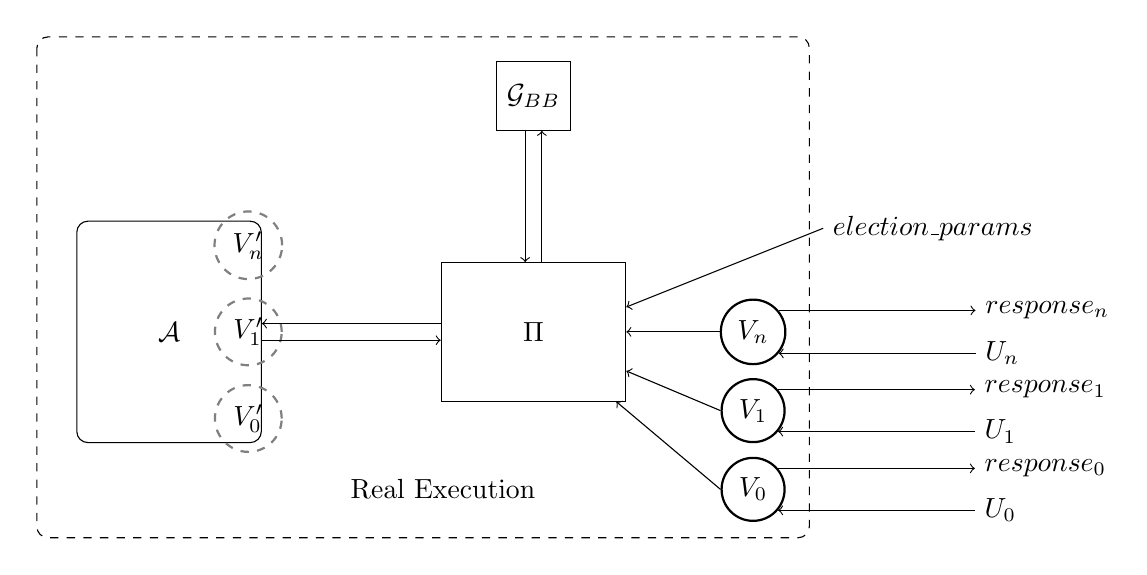
\begin{tikzpicture}
    \node (s) [a] {$\mathcal{A}$};
    \path (s.east)+(1.5*\blockdist,3) node (g) [sensor] {$\mathcal{G}_{BB}$};
    \path (s.east)+(1.5*\blockdist,0) node (system) [s] {$\Pi$};
    \path (system.east) +(0.7*\blockdist,-2) node (v0) [v] {$V_0$};
    \path (system.east) +(0.7*\blockdist,-1) node (v1) [v] {$V_1$};
     \path (system.east) +(0.7*\blockdist, 0) node (vn) [v] {$V_n$};
     \path (s.west) +(0.95*\blockdist,-1.1) node (v0') [vv] {$V_0'$};
      \path (s.west) +(0.95*\blockdist,0) node (v1') [vv] {$V_1'$};
       \path (s.west) +(0.95*\blockdist,1.1) node (vn') [vv] {$V_n'$};
    \path (s.east) +(\blockdist, -2) node (RE) {Real Execution};
    \draw[transform canvas={yshift=0.7ex},->] (system) -- (s);
    \draw[transform canvas={yshift=-0.7ex},<-] (system) -- (s);
    \draw[transform canvas={xshift=0.7ex},->] (system) -- (g);
    \draw[transform canvas={xshift=-0.7ex},<-] (system) -- (g);
     \path [draw, <-] (system) --  (v1.west);
      \path [draw, <-] (system) -- (v0.west);
      \path [draw, <-] (system) --  (vn.west);
    \draw [<-] (v0.-40)-- node [ann] {} + (\edgedist,0) 
        node[right] {$U_0$};
      \draw [<-] (v1.-40)-- node [ann] {} + (\edgedist,0) 
        node[right] {$U_1$};
     \draw [<-] (vn.-40)-- node [ann] {} + (\edgedist,0) 
        node[right] {$U_n$};
     \draw [->] (v0.40)-- node [ann] {} + (\edgedist,0) 
        node[right] {$response_0$};
      \draw [->] (v1.40)-- node [ann] {} + (\edgedist,0) 
        node[right] {$response_1$};
     \draw [->] (vn.40)-- node [ann] {} + (\edgedist,0) 
        node[right] {$response_n$};
        \draw [<-] (system.15) -- node [ann] {} + (\edgedist,1) 
        node[right] {$election\_params$};
    \begin{pgfonlayer}{background}
        \path (s.west |- g.north)+(-0.5,0.3) node (a) {};
        \path (v0.south -| v0.east)+(+0.3,-0.2) node (b) {};
        \path[rounded corners, draw=black, dashed]
            (a) rectangle (b);
    \end{pgfonlayer}
\end{tikzpicture}
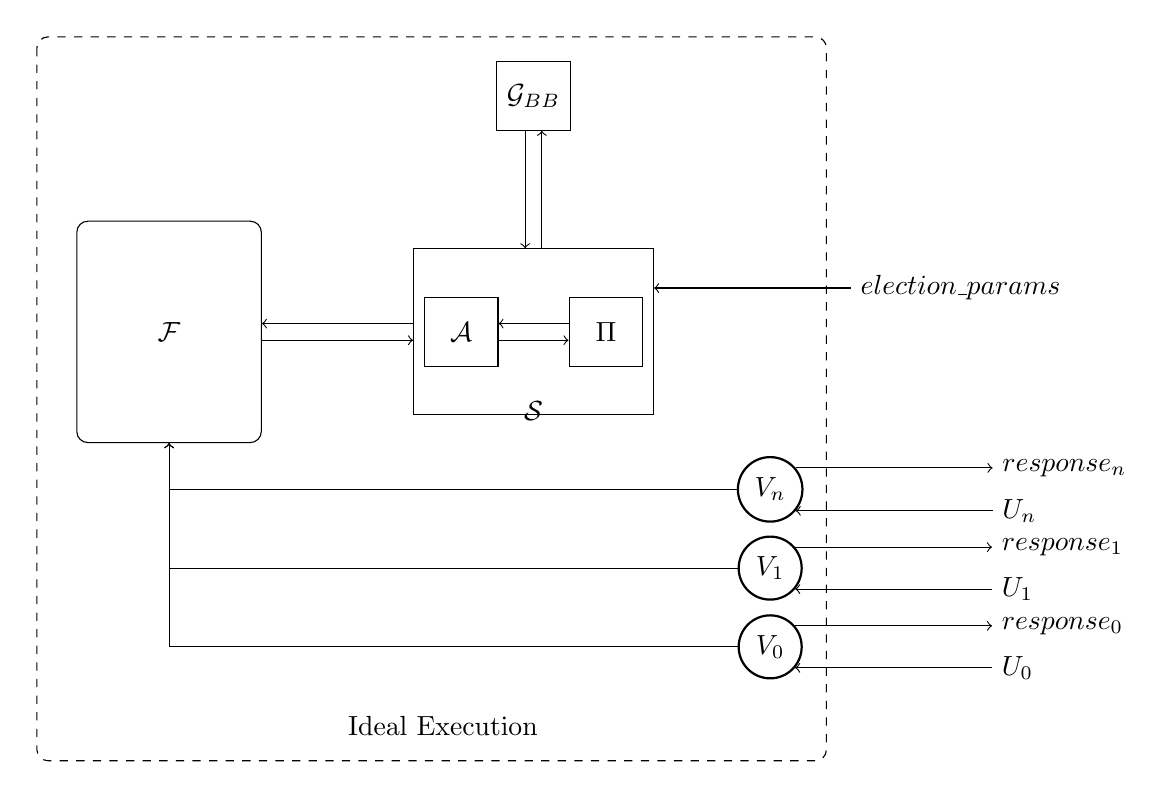
\begin{tikzpicture}
    \node (s) [a] {$\mathcal{F}$};
    \path (s.east)+(1.5*\blockdist,3) node (g) [sensor] {$\mathcal{G}_{BB}$};
    \path (s.east)+(1.5*\blockdist,0) node (system) [sim] {};
    \path (s.east)+(1.1*\blockdist,0) node (adv) [sensor] {$\mathcal{A}$};
     \path (s.east)+(1.9*\blockdist,0) node (ss) [sensor] {$\Pi$};
    \path (ss.east) +(0.7*\blockdist,-4) node (v0) [v] {$V_0$};
    \path (ss.east) +(0.7*\blockdist,-3) node (v1) [v] {$V_1$};
     \path (ss.east) +(0.7*\blockdist, -2) node (vn) [v] {$V_n$};
    \path (s.east) +(\blockdist, -5) node (RE) {Ideal Execution};
     \path (s.east) +(1.5*\blockdist, -1) node (ssimulator) {$\mathcal{S}$};
    \draw[transform canvas={yshift=0.7ex},->] (system) -- (s);
    \draw[transform canvas={yshift=-0.7ex},<-] (system) -- (s);
    \draw[transform canvas={xshift=0.7ex},->] (system) -- (g);
    \draw[transform canvas={xshift=-0.7ex},<-] (system) -- (g);
    \draw[transform canvas={yshift=0.7ex},->] (ss) -- (adv);
    \draw[transform canvas={yshift=-0.7ex},<-] (ss) -- (adv);
     \path [draw, <-] (s) |-  (v1.west);
      \path [draw, <-] (s) |- (v0.west);
      \path [draw, <-] (s) |-  (vn.west);
    \draw [<-] (v0.-40)-- node [ann] {} + (\edgedist,0) 
        node[right] {$U_0$};
      \draw [<-] (v1.-40)-- node [ann] {} + (\edgedist,0) 
        node[right] {$U_1$};
     \draw [<-] (vn.-40)-- node [ann] {} + (\edgedist,0) 
        node[right] {$U_n$};
     \draw [->] (v0.40)-- node [ann] {} + (\edgedist,0) 
        node[right] {$response_0$};
      \draw [->] (v1.40)-- node [ann] {} + (\edgedist,0) 
        node[right] {$response_1$};
     \draw [->] (vn.40)-- node [ann] {} + (\edgedist,0) 
        node[right] {$response_n$};
        \draw [<-] (system.20)-- node [ann] {} + (\edgedist,0) 
        node[right] {$election\_params$};
    \begin{pgfonlayer}{background}
        \path (s.west |- g.north)+(-0.5,0.3) node (a) {};
        \path (RE.south -| v0.east)+(+0.3,-0.2) node (b) {};
        \path[rounded corners, draw=black, dashed]
            (a) rectangle (b);
    \end{pgfonlayer}
\end{tikzpicture}
        \caption{Real and Ideal Execution}
        \label{ RI}
\end{figure}\\
Security requires existence of some simulator program $\mathcal{S}$ such that the real and ideal executions are indistinguishable for and any environment  $\mathcal{Z}$. Unfortunately, as we are about to show, no such simulator exists.\\\\
\textbf{Proposition:}\\ 
For any system $\Pi$ that satisfies the definition of strict privacy, there is an adversary $\mathcal{A}$  such that for any simulator $\mathcal{S}$, there is an environment $\mathcal{Z}$ that distinguishes ideal and real executions $\exec_{\mathcal{Z}, \mathcal{S}}^{\mathcal{F}, \mathcal{G}_{BB}} \not \approx \exec_{\mathcal{Z},\mathcal{A}}^{\Pi, \mathcal{G}_{BB}}$ \\\\
\subsection{Proof: part 1}
Suppose we have a system $\Pi$, which is strictly private in case ``$\ea$ is corrupted, but $\vsd$ is honest".\\
Consider the following attack against E2E Verifiability: \\
\fbox{\begin{minipage}{30em}
$\mathcal{A}$:\\
-- corrupts $\ea$ and $\vsd$s but doesn't corrupt $\asd$s.\\
-- corrupts $t$ voters $(t \leq n)$ , where $n$ is the total number of voters.\\ 
-- creates fake voters $\{V_0',V_1',\dots,V_n'\}$ and using its power substitutes some part $\gamma$ of honest voters with fake ones for the $U_a$ option.\\
-- fake voters vote for adversarial options according to a vote-casting procedure.\\
-- substituted honest voters receive receipts generated for fake voters.
\end{minipage}}\\\\
  \begin{figure}[h!]
 \includestandalone[mode=buildnew]{figures/attack}
        \caption{  $\mathcal{A}$}
\end{figure}\\
let $\mathcal{Z}$ be the environment that works as follows:\\\\
\fbox{\begin{minipage}{30em}
$\mathcal{Z}$:\\
--  defines an election setup information:\\ $election\_params = (\mathcal{C},\mathcal{V}, \mathcal{U}, params)$, where $\mathcal{C}$ - list of candidates, $\mathcal{V}$ - list of voters, $\mathcal{U}$ - list of allowed candidates' selections, $params$ - other required information.\\
-- instructs each voter $V_i$ to vote for the blank $`no~one'$ option.\\
-- stops the vote-casting phase.\\
-- asks $\mathcal{G}_{BB}$ for the election result $\tau$\\
--  asks every voter $V_i$ to verify his choice and return the result of verification - $response_i$, where $response_i$ equal to $(sid, verify\_responce, \tau')$  in case of successful verification and $\bot$ otherwise.\\
-- If the number of successful verification responses equal to the number of voters and in all responses provided by a voter tally $\tau'$ is equal to the $\mathcal{G}_{BB}$'s tally $\tau$ return 1. Otherwise return 0.
\end{minipage}}
\\\\
 Since $\Pi$ is strictly private, probability, that an adversary $\mathcal{D}$ engaging in the \textbf{Cast} protocol would distinguish real and simulated view and win the attack against the strict privacy $Pr[G_{strict,\vsd,T}^{\mathcal{D},Sim}(1^{\lambda}) = 1] = \frac{1}{2} + \alpha$ where $\alpha$ is negligible. In case of corrupted $\ea$, $\mathcal{C}$ returns a real ballot and receipt pair and a simulated via $Sim$ pair. This means that in a strictly private system an adversary has a negligible chance to distinguish the ballot and receipt for his option and for some $U_c$ option. \\\\
During the Real Execution a voter can either accept or reject the cast ballot. Rejection is possible only if he detects that the receipt and ballot are faked. The probability that a voter distinguish the receipt and ballot for his option from for the `no-one' option and rejects is $\Pr[V_i~rejects] \leq  \alpha$, where $\alpha$ is negligible.\\\\
 By nature of the attack $\mathcal{A}$,  fake receipt is the perfectly valid receipt for the $U_a$ option and the cast ballot would always be successfully verified. Therefore in the Real Execution $\mathcal{Z}$ would get a successful verification response from all n voters and output 1 with the probability $\Pr[\exec_{\mathcal{Z},\mathcal{A}}^{\Pi, \mathcal{G}_{BB}} = 1] =  \Pr[all~V_i~accept] = \prod_{i=0}^n(1- \Pr[V_i~rejects] ) \geq (1 - \alpha)^n = 1 - n\alpha = 1- \beta$, where $\beta = n\alpha $ is negligible. Thus, $\Pr[\exec_{\mathcal{Z},\mathcal{A}}^{\Pi, \mathcal{G}_{BB}} = 0] = 1 - \Pr[\exec_{\mathcal{Z},\mathcal{A}}^{\Pi, \mathcal{G}_{BB}} = 1] \leq \beta$, where $\beta$ is negligible.\\\\
Suppose for the sake of contradiction that $\Pr[\exec_{\mathcal{Z},\mathcal{A}}^{\Pi, \mathcal{G}_{BB}} = 0] \geq  \beta$, where $\beta$ is non-negligible. This means that at least one voter rejects the receipt. I will show that this contradicts the definition of strict privacy. Consider an attacker $\mathcal{B}$ against strict privacy which exploits the environment  $\mathcal{Z}$. \\\\
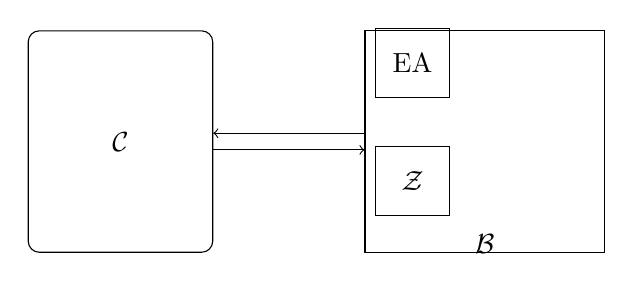
\begin{tikzpicture}
    \node (s) [a] {$\mathcal{C}$};
    \path (s.east)+(1.5*\blockdist,0) node (system) [draw, text width=8em, 
    text centered, minimum height=8em] {};
    \path (s.east)+(1.1*\blockdist,1) node (adv) [sensor] {$\ea$};
     \path (s.east)+(1.1*\blockdist,-0.5) node (ss) [sensor] {$\mathcal{Z}$};
     \path (s.east) +(1.5*\blockdist, -1.3) node (ssimulator) {$\mathcal{B}$};
    \draw[transform canvas={yshift=0.7ex},->] (system) -- (s);
    \draw[transform canvas={yshift=-0.7ex},<-] (system) -- (s);
\end{tikzpicture}

\fbox{\begin{minipage}{30em}
$\mathcal{B}$ interacts with the challenger in the strict privacy attack  $\mathcal{C}$ as follows: \\
-- $\mathcal{Z}$ defines an election parameters  $election\_params$, assign every voter to vote for the blank option $\{V_i,`no~one'\}$ and send this information to the $\mathcal{B}$.\\
-- $\mathcal{B}$ forwards received $election\_params$ to the $\ea$. \\
-- $\mathcal{B}$ corrupts the $\ea$.\\
-- $\ea$ starts the election.\\
-- $\mathcal{B}$ interacts with the challenger $\mathcal{C}$ provides  $(V_i,`no~one',U_{\mathcal{Z}_i})$ as the input.\\ 
--  $\mathcal{C}$ sends back to the $\mathcal{B}$ real and simulated view $(b_0,r_0), (b_1,r_1)$ in the order defined by the challenger's coin a. \\
-- $\mathcal{B}$ votes on behalf of all voters\\
-- $\mathcal{Z}$ stops the vote-casting phase.\\
--  $B$ computes the election's tally and proof of the tally's correctness.\\
-- $\mathcal{Z}$ asks $\mathcal{G}_{BB}$ for the election result $\tau$\\
-- $\mathcal{Z}$ requests every voter to verify his ballot correctness.\\
-- $\mathcal{B}$ will run the verification on behalf of all voters using ballots and receipts from $\{b_0,r_0\}$.\\
-- $\mathcal{Z}$ outputs 1 or 0 depending on the voters' verdict.\\
--$\mathcal{B}$ outputs whatever the $\mathcal{Z}$ outputs.
\end{minipage}}\\\\
The challenger $\mathcal{C}$  outputs simulated ballot and receipt as $(b_0,r_0)$, when the coin $a=0$ and as $(b_1,r_1)$ otherwise.\\\\
In case when $a=0, \mathcal{B}$'s behaviour is identical to the $\mathcal{A}$'s strategy and $\mathcal{B}$ wins if $\mathcal{Z}$ outputs 0, which happens if at least one voter rejects the simulated receipt.  By assumption $\Pr[\exec_{\mathcal{Z},\mathcal{A}}^{\Pi, \mathcal{G}_{BB}} = 0] \geq  \beta$, where $\beta$ is non-negligible. Therefore if $(b_0,r_0)$ is the set of simulated ballot and receipt, $\mathcal{B}$ wins with the probability $Pr[\mathcal{B} \rightarrow 0| a=0] = \Pr[\exec_{\mathcal{Z},\mathcal{A}}^{\Pi, \mathcal{G}_{BB}}~=~0] \geq \beta$, where $\beta$ is non-negligible. \\\\
On the other hand, when $a=1$, $\mathcal{B}$ plays honestly and the probability of $\mathcal{Z}$ outputting 1 is equal to probability that all voters successfully verify their votes in the honest execution, which is happens with overwhelming probability $1-negl(\lambda)$.\\\\ 
The probability of $\mathcal{B}$  winning the attack against the strict privacy is \\$\Pr[G_{strict}^{\mathcal{B}}(1^{\lambda})=1]= \Pr[\mathcal{B} \rightarrow 0| a=0]\Pr[a=0] + \Pr[\mathcal{B} \rightarrow 1| a=1]\Pr[a=1] =  \Pr[\exec_{\mathcal{Z},\mathcal{A}}^{\Pi, \mathcal{G}_{BB}}=0]\Pr[a=0]  + \Pr[\exec_{\mathcal{Z},honest}^{\Pi, \mathcal{G}_{BB}} =1]\Pr[a=1] \geq \frac{1}{2}\beta+ \frac{1}{2} - negl(\lambda)$ , where $\beta$ is not negligible. This implies that $\mathcal{B}$ wins the attack against strict privacy with the probability more than $\frac{1}{2} + negl(\lambda)$, which contradicts the assumption that the $\Pi$ is strictly private.\\\\
In the Ideal Execution any simulator $S$ can either:\\
1) post in $\mathcal{G}_{BB}$ the tally $\tau'$ generated by $\mathcal{A}$ or any other tally  $\tau' \neq \tau$\\ 
or\\
2) ignore the $\mathcal{A}$'s tally and post the actual tally $\tau$.\\\\
In the first case, the ideal functionality for E2E verifiability  $\mathcal{F}$  would always detect the tally deviation caused by $\mathcal{A}$ if such exists. And since  $\mathcal{A}$ doesn't corrupt $\asd$s, for all honest voters the ideal functionality $\mathcal{F}$ would block verification responses. This implies that in the Ideal Execution $\exec_{\mathcal{Z}, \mathcal{S}}^{\mathcal{F}, \mathcal{G}_{BB}}$ $\mathcal{Z}$ would get no response from honest voters. The total number of successful verifications would be equal to the number of corrupted voters, which is less (if not voters are corrupted) than the total number of voters -- $\mathcal{Z}$ outputs 0.  \\\\
In the second case, there exists a class of simulators which ignore $\mathcal{A'}$ actions and post the actual tally.  For those simulators consider an modified  environment $\tilde{\mathcal{Z}}$ that works as follows:\\\\
\fbox{\begin{minipage}{33em}
$\tilde{\mathcal{Z}}$:\\
Outputs a bit according to the following rules:\\
$ \begin{cases}
 \text{if} ~~\mathcal{Z}~~ \text{outputs 1 and the number of non-blank votes greater or equal}~~ \gamma \text{-- output 1} \\ 
 \text{else output 0}
\end{cases}$
\end{minipage}}.
$\tilde{\mathcal{Z}}$ would still output 1 in case of the real execution since the number of non-blank votes would be at least $\gamma$ due to successful attack  $\mathcal{A}$. However  $\tilde{\mathcal{Z}}$ would not find at least $\gamma$ non-blank votes and output 0 in the ideal execution. \\\\
Thus, there is the attacker $\mathcal{A}$ such that for any simulator $\mathcal{S}$ there is the environment $\tilde{\mathcal{Z}}$ or $\mathcal{Z}$ which can always distinguish real and ideal executions. \\\\
\subsection{Proof: part 2}
Suppose we have a system $\Pi'$, which is strictly private in case ``$\ea$ is honest, but $\vsd$ is corrupted".\\
Consider the following attack against E2E Verifiability: \\
\fbox{\begin{minipage}{30em}
$\mathcal{A'}$:\\
-- corrupts $\ea$ and $\vsd$s but doesn't corrupt $\asd$s.\\
-- chooses an option $U_a \in \mathcal{U}$\\
-- corrupts $t$ voters $(t \leq n)$ , where $n$ is the total number of voters.\\ 
-- provides every honest voter $V_i$ with fake credentials $s_i'$ s.t. the ballot and receipt produced using $(s_i',`no~one')$ are identical to the ballot and receipt produced using real credentials for an option $U_a$: $b,r \leftarrow (s_i',`no~one') $ AND $ b,r \leftarrow (s_i,U_a)$\\
-- creates fake voters $\{V_0',V_1',\dots,V_n'\}$ and provides them with real credentials $s_i$\\
--  using its power substitutes some part $\gamma$ of honest voters' cast protocols with the fake voters' protocols for the $U_a$ option.
\end{minipage}}\\\\
let $\mathcal{Z'}$ be the environment that works as follows:\\\\
\fbox{\begin{minipage}{30em}
$\mathcal{Z'}$:\\
--  defines an election setup information:\\ $election\_params = (\mathcal{C},\mathcal{V}, \mathcal{U}, params)$, where $\mathcal{C}$ - list of candidates, $\mathcal{V}$ - list of voters, $\mathcal{U}$ - list of allowed candidates' selections, $params$ - other required information.\\
-- instructs each voter $V_i$ to vote for the blank option (`no~one').\\
-- stops the vote-casting phase.\\
-- asks $\mathcal{G}_{BB}$ for the election result $\tau$\\
--  asks every voter $V_i$ to verify his choice and return the result of verification - $response_i$, where $response_i$ equal to $(sid, verify\_responce, \tau')$  in case of successful verification and $\bot$ otherwise.\\
-- If the number of successful verification responses equal to the number of voters and in all responses provided by a voter tally $\tau'$ is equal to the $\mathcal{G}_{BB}$'s tally $\tau$ return 1. Otherwise return 0.
\end{minipage}}
\\\\
Since $\Pi'$ is strictly private, probability, that an adversary engaging in the \textbf{Registration} protocol would distinguish real and simulated view and win the attack against the strict privacy $|\Pr[G_{strict,\ea}^{\mathcal{A},Sim}(1^{\lambda}) = 1] - \frac{1}{2}| = \alpha$ where $\alpha$ is negligible. In case ``$\ea$ is honest, but $\vsd$ is corrupted'', simulated view is credentials $\tilde{s_i}$ generated via the simulator $Sim$. \\\\
%%%%%
In the Real Execution a voter $V_i$ starts the Cast protocol using fake credentials $s_i'$ and an option $`no~one'$. However, $\mathcal{A'}$ substitutes his ballot and receipt with the ballot and receipt generated for a fake voter with real credentials and $U_a$ option. By nature of the attack, the returned receipt generated for real credentials and the $U_a$ option is identical to the receipt produced for a fake credentials and $`no~one'$ option. Therefore in the Real Execution $\mathcal{Z'}$ would output 1 if non of the voters would detect that he was given a receipt for fake credentials. The probability of this event is $\Pr[\exec_{\mathcal{Z'},\mathcal{A'}}^{\Pi', \mathcal{G}_{BB}} = 1] =  \Pr[all~V_i~accept] = \prod_{i=0}^n(1- \Pr[V_i~rejects] )$. Suppose, the probability of rejection by $V_i$ is $ \Pr[V_i~rejects] = \zeta$. Thus,   $\Pr[\exec_{\mathcal{Z'},\mathcal{A'}}^{\Pi', \mathcal{G}_{BB}} = 1] = (1 - \zeta)^n = 1 - n\zeta = 1- \zeta'$.\\\\
%%%%
Suppose that $ \zeta'$ is not negligible. This means that $\Pr[\exec_{\mathcal{Z'},\mathcal{A'}}^{\Pi', \mathcal{G}_{BB}} = 0] = 1 - \Pr[\exec_{\mathcal{Z'},\mathcal{A'}}^{\Pi', \mathcal{G}_{BB}} = 1] =  \zeta'$, where $ \zeta'$ is not negligible. This means that at least one voter rejects the receipt with a non-negligible probability. We will show that this contradicts the definition of strict privacy. Consider an attacker $\mathcal{B'}$ against strict privacy which exploits the environment  $\mathcal{Z'}$. \\\\
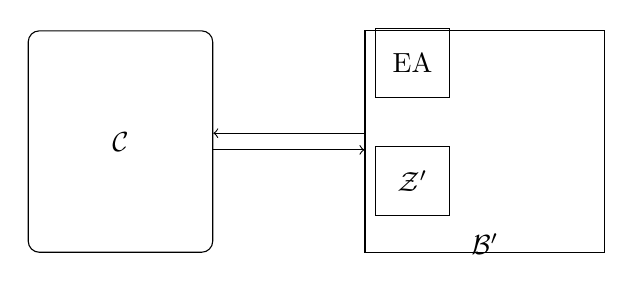
\begin{tikzpicture}
    \node (s) [a] {$\mathcal{C}$};
    \path (s.east)+(1.5*\blockdist,0) node (system) [draw, text width=8em, 
    text centered, minimum height=8em] {};
    \path (s.east)+(1.1*\blockdist,1) node (adv) [sensor] {$\ea$};
     \path (s.east)+(1.1*\blockdist,-0.5) node (ss) [sensor] {$\mathcal{Z'}$};
     \path (s.east) +(1.5*\blockdist, -1.3) node (ssimulator) {$\mathcal{B'}$};
    \draw[transform canvas={yshift=0.7ex},->] (system) -- (s);
    \draw[transform canvas={yshift=-0.7ex},<-] (system) -- (s);
\end{tikzpicture}\\\\
\fbox{\begin{minipage}{30em}
$\mathcal{B'}$ interacts with the challenger in the strict privacy attack  $\mathcal{C}$ as follows: \\
-- $\mathcal{Z}$ defines an election parameters  $election\_params$, assign each voter the blank option $\{V_i,`no~one'\}$ and send this information to the $\mathcal{B}$.\\
-- $\mathcal{B'}$ forwards received $election\_params$ to the $\mathcal{C}$. \\
-- $\mathcal{B'}$ corrupts the $\vsd$.\\
-- $\mathcal{C}$ starts the election.\\
-- $\mathcal{B'}$ sends  to $\mathcal{C}$ $(V_i,`no~one',U_a)$.\\
-- $\mathcal{C}$ sends back $s_0,s_1$. \\
--  $\mathcal{B'}$ provides voters with credentials $s_0$ and uses $(s_0,`no~one')$ to produce the ballot and receipt and posts the result on $\bb$.\\ 
-- $\mathcal{Z'}$ stops the vote-casting phase.\\
--  $\mathcal{C}$ executes the $Tally$ protocol.\\
-- $\mathcal{Z'}$ asks $\mathcal{G}_{BB}$ for the election result $\tau$\\
-- $\mathcal{Z'}$ requests every voter to verify his ballot correctness.\\
-- $\mathcal{B'}$ will run the verification on behalf of all voters.\\
-- $\mathcal{Z'}$ outputs 1 or 0 depending on the voters' verdict.\\
-- $\mathcal{B'}$ outputs whatever the $\mathcal{Z'}$  outputs.\\
\end{minipage}}\\\\
In case when the simulated credentials are chosen ($a=0$), $\mathcal{B'}$ provides a voter with fake credentials and generated ballot and receipt for the blank option using the fake credentials, which means that real credentials correspond to the $U_a$ option. $\mathcal{B'}$'s behaviour is identical to the $\mathcal{A'}$'s strategy. $\mathcal{B'}$ wins if outputs 0, which happens if  $\mathcal{Z'}$ outputs 0. $\Pr[\mathcal{B}'\rightarrow 0| a=0 ] = \Pr[\exec_{\mathcal{Z'},\mathcal{A'}}^{\Pi', \mathcal{G}_{BB}}=0] = \zeta'$\\\\
%
Else if $a=1$, $\mathcal{B'}$ provides a voter with real credentials and uses the real credentials to vote for the blank option, which is honest behaviour. $\Pr[B'\rightarrow 1| a=1] =\Pr[\exec_{\mathcal{Z'},honest}^{\Pi', \mathcal{G}_{BB}}=1] = 1$\\\\
%
Thus, the probability of $\mathcal{B'}$  winning the attack against the strict privacy is \\$\Pr[G_{strict,\ea}^{\mathcal{B}, Sim}(1^{\lambda})=1]= \frac{1}{2}(\Pr[B'\rightarrow 0| a=0] + \Pr[B'\rightarrow 1| a=1])  = \frac{1}{2} (\zeta' +1) =  \frac{1}{2}  +  \frac{1}{2} \zeta'$ , where $\zeta'$ is not negligible. This implies that $\mathcal{B'}$ wins the attack against strict privacy with the probability more than $\frac{1}{2} + negl(\lambda)$, which contradicts the assumption that the $\Pi$ is strictly private.\\\\
In the Ideal Execution any simulator $S$ can either:\\
1) post in $\mathcal{G}_{BB}$ the tally $\tau'$ generated by $\mathcal{A'}$ or any other tally  $\tau' \neq \tau$\\ 
or\\
2) ignore the $\mathcal{A'}$'s tally and post the actual tally $\tau$.\\\\
In the first case, the ideal functionality for E2E verifiability  $\mathcal{F}$  would always detect the tally deviation caused by $\mathcal{A'}$ if such exists. And since  $\mathcal{A'}$ doesn't corrupt $\asd$s, for all honest voters the ideal functionality $\mathcal{F}$ would block verification responses. This implies that in the Ideal Execution $\exec_{\mathcal{Z'}, \mathcal{S}}^{\mathcal{F}, \mathcal{G}_{BB}}$ $\mathcal{Z'}$ would get no response from honest voters. The total number of successful verifications would be equal to the number of corrupted voters, which is less (if not voters are corrupted) than the total number of voters -- $\mathcal{Z'}$ outputs 0.  \\\\
In the second case, there exists a class of simulators which ignore $\mathcal{A'}$ actions and post the actual tally.  For those simulators consider an modified  environment $\tilde{\mathcal{Z'}}$ that works as follows:\\
\fbox{\begin{minipage}{33em}
$\tilde{\mathcal{Z'}}$:\\
Outputs a bit according to the following rules:\\
$ \begin{cases}
 \text{if} ~~\mathcal{Z}~~ \text{outputs 1 and the number of non-blank votes greater or equal}~~ \gamma \text{-- output 1} \\ 
 \text{else output 0}
\end{cases}$
\end{minipage}}.
$\tilde{\mathcal{Z'}}$ would still output 1 in case of the real execution since the number of non-blank votes would be at least $\gamma$ due to successful attack  $\mathcal{A}$. However  $\tilde{\mathcal{Z'}}$ would not find at least $\gamma$ non-blank votes and output 0 in the ideal execution. \\\\
Thus, there is the attacker $\mathcal{A'}$ such that for any simulator $\mathcal{S}$ there is the environment $\tilde{\mathcal{Z'}}$ or $\mathcal{Z'}$ which can always distinguish real and ideal executions. 
\section {Blind signature e-voting scheme}
Here is the description of a blind signature e-voting system for 1-out-of-m elections.\\
The Blind signature scheme 
\textbf{Setup ($1^{\lambda}, \mathcal{P} = \{P_1,\dots,P_m\}, \mathcal{V} = \{V_1,\dots,V_n\}, \mathcal{U} =  \{\{P_1\},\dots,\{P_m\}\})$.}\\\\
Let ($GenBL, EncrB, SignBL)$ be the PPT algorithms that constitutive the RSA blind signature scheme,  $PRG_{str}$  - a function for pseudo random string generation, $PRG_{prime}$  - a function for pseudo-random prime number generation and $(Gen, Encr, Decr)$ - PPT algorithms for the ELGamal encryption scheme. The EA runs $GenBL(Param, 1^{\lambda})$ to generate the blind signature scheme keys $(bsk, bpk)$ and $Gen(Param, 1^{\lambda})$ to generate ELGamal keys $(sk,pk)$. Public keys $bpk,pk$ and functions $EncrB,Encr, PRG_{str}, PRG_{prime}$ are posted on the BB.\\
Then, for every voter $V_l$, where $l \in [n]$, EA runs $PRG_{str}(1^{\lambda})$ function to generate random string $seed_l$.\\\\
\textbf{Registration}\\\\
Let $(GenAES, EncrAES, DecrAES)$ be the publicly known PPT algorithms that implements AES encryption scheme and $Hash$ - hash algorithm.  \\\\
Every voter $V_l$ completes the following procedure: \\
--  uses the published on the BB function $PRG_{str}(1^{\lambda})$ to generate his alias $x_l$ and  $PRG_{prime}(bpk)$ to generate a blinding factor $z_l$. \\
-- calculates value $p_l = Hash(x_l)EncrB(z_l)$.\\
--  chooses his secret password $password_l$ and runs  $ GenAES(password_l, s_l)$ to generate his key for symmetric encryption $key_l$, where $s_l = PRG_{str}(seed_l)$.\\
--  encrypts $x_l$ and $z_l$ by running  $EncrAES(key_l,x_l)$ and $EncrAES(key_l,z_l)$ respectively to get encrypted values $\hat{x_l},\hat{z_l}$\\
-- sends $p_l,\hat{x_l},\hat{z_l}$ to the EA\\\\
 EA:\\
Upon receiving $p_l,\hat{x_l},\hat{z_l}$ from a voter, EA posts all information to the BB.\\
When registration is closed, EA runs  $SignBL(bsk, p_l)$ for every entry in the BB and post the result in the corresponding line as $p^{sign}_l$.\\\\
\textbf{Cast:}\\
Let $e_l = (e_{1_l},e_{2_l},\dots,e_{m_l})$ be the characteristic vector corresponding to the voter's selection, where $e_{j_l}=1$ if the option $opt_j$ is selected by the voter $V_l$.\\ 
Every voter $V_l$ completes the following procedure:\\
-- gets all information from the BB - $\{p_l,\hat{x_l},\hat{z_l}\}$.\\
-- finds his entry and decrypts $x_l$ and $z_l$ by running $DecrAES(key_l,\hat{x_l})$ and $DecrAES(key_l,\hat{z_l})$ respectively, where $key_l =  GenAES(password_l, s_l)$ and  $s_l = PRG_{str}(seed_l)$\\
-- computes  $\sigma_l$ - signature for $x_l$  by calculating  $p^{signed}_lz_l^{-1}$\\
-- computes $\Pi_l$ -- NIZK proof of signature knowledge .\\
-- chooses his vote-option $e_{j_l}$ and writes the corresponding characteristic vector $e_l$\\
-- for $j \in [m]$ compute $c_{j_l} =  Encr(pk,e_{j_l})$\\
-- computes NIZK proofs $\pi_{j_l}$ that each $c_{j_l}$ is an encryption of 1 or 0.\\
-- sends $b_l = (x_l, \sigma_l, \Pi_l, c_l, \pi_l)$ to the EA.\\
-- keeps $x_l$ as receipt.\\
-- If EA accept $b_l$, protocol terminates successfully.\\ 
*Optional: every voter can export the randomness to check that the ballot was cast as intended.\\\\
Upon receiving $(x_l, \sigma_l, \Pi_l, c_l, \pi_l)$ from a voter, EA checks NIZK proofs and, if it's valid, accepts the ballot and posts all information to the BB.\\\\
\textbf{Tally: }\\
After election is closed, EA computes $\mathcal{C}$ -- the sum of all $c_l$ and runs $Decr(sk, \mathcal{C})$ to decrypt Tally $\tau$. EA posts the $\tau$ along with the proof of tally correctness $Proof$.\\\\
\textbf{Result:} \\
result is straightforward.\\\\
\textbf{Verify:} \\
The algorithm returns 1 only if the following checks are true:\\
--  exported randomness is correct or voter choose not to check.\\
-- there is ballot with $x_l$\\
-- all $\Pi_l, \pi_l$ are valid\\
-- number of ballots less or equal to the number of registered voters\\
-- $Proof$ is correct\\
-- sum of all scores at $\tau$ are less than or equal to ballot numbers\\\\
\textbf{Construction of the vote extractor.}\\ 
$\mathcal{E}$ has input $\tau$ and the set of receipts  $\{x_l\}_{V_l \in \tilde{\mathcal{V}}}$ where $\tilde{\mathcal{V}}$ is the set of the honest voters that voted successfully.  If $Result(\tau) = \perp$ (i.e., the transcript is not meaningful), then $\mathcal{E}$ outputs $\perp$. Otherwise, $\mathcal{E}$ (arbitrarily) arranges the voters in $\mathcal{V} \backslash \tilde{\mathcal{V}}$ and the tags not included in $\{x_l\}_{V_l \in \tilde{\mathcal{V}}}$ as $\langle V_l^{\mathcal{E}} \rangle_{l \in  [n - |\tilde{\mathcal{V}}|]}$ and $\langle tag_l^{\mathcal{E}} \rangle_{l \in  [n - |\tilde{\mathcal{V}}|]}$ respectively. Next, for every $l \in [n - |\tilde{\mathcal{V}}|]$:\\
\begin{enumerate}
\item  $\mathcal{E}$ finds at the BB entry with   $x_l = tag_l^{\mathcal{E}}$ and brute-force the corresponding ELGamal cipher to open the selected candidate $\mathcal{P}_l^{\mathcal{E}}$. If $\mathcal{P}_l^{\mathcal{E}}$ is the valid candidate's selection, then $\mathcal{E}$ sets $\mathcal{U}_l^{\mathcal{E}} = \{\mathcal{P}_l^{\mathcal{E}}\}$. Otherwise it inputs $\perp$.
\end{enumerate}
Finally $\mathcal{E}$ outputs  $\langle \mathcal{U}_l^{\mathcal{E}} \rangle_{V_l \in \mathcal{V} \backslash \tilde{\mathcal{V}}  }$
\end{document}